% arara: xelatex: { shell: true, interaction: nonstopmode } if changed('tex') || changed(toFile('fefudoc.cls'))
%arara: biber if changed('bib') || changed('bcf') || changed('bbl')
%arara: xelatex: { synctex: true, shell: true } if changed('aux')
% !TeX document-id = {bee52599-d588-4a9f-9dfb-bb5e4a21d678}
% !TeX program = xelatex
% !TeX encoding = UTF-8
% !TeX spellcheck = ru_RU
% !TeX TXS-program:compile=txs:///xelatex/[--shell-escape]|txs:///view-pdf
% !TeX TXS-program:bibliography = txs:///biber
\documentclass[ {{barchelor thesis}}, draught ]{fefudoc}
\usepackage{enumitem} %нумерованные списки
\usepackage{amsmath, amsfonts, amssymb, mathtools} %математика
\usepackage{tikz} %рисование
\usetikzlibrary{positioning, calc, arrows, decorations.markings}
\usepackage[siunitx]{circuitikz} %рисование логических и принципиальных схем
\usepackage{makecell} %доп. форматирование ячеек таблиц
\renewcommand\theadfont{\normalsize\bfseries} %сделать заголовки таблиц из makecell
\usepackage{biblatex} %список литературы
\addbibresource{./главы примеров ВКР/список литературы.bib} %Файл со списком литературы.
\usepackage{longtable, multirow} %длинные таблицы и многострочные ячейки
\usepackage{pdflscape} %временное изменение ориентации страниц
\usepackage{listings} %программный код
\lstset{ %общие параметры расширения listings
	basicstyle=\ttfamily\small, %выделять код программ специальным шрифтом малого размера
	keywordstyle=\bfseries, %выделять ключевые слова языка жирным начертанием
	commentstyle=\itshape, %выделять комментарии курсивом
	columns=flexible, %сжимать при необходимости межсимвольный интервал для умещения на странице
	frame=single, %обводить программный код одинарной рамкой
	tabsize=2 %табуляция в программном коде эквивалентна двум пробелам
}

\Institute{Институт математики и компьютерных технологий (Школа)}
\Department{Департамент программной инженерии и искусственного интеллекта}
\specialty{09.03.04}
\profile{Программная инженерия}
\location{Владивосток}
 
\author{Б9119-09.03.04прогин}{Андреев Борис Викторович}
\tutor{кандидат технических наук}{}{доцент департамента ЭТиП}{Борисов Виктор Геннадиевич}
%\reviewer{кандидат технических наук}{}{}{Викторов Геннадий Дмитриевич}
%\normcontrol{}{}{}{Геннадиев Дмитрий Евгеньевич}
\exportcontrol{}{}{}{Дмитриев Евгений Жаннович}
\secretary{}{}{}{Евгениев Жан Захарович}
\superintendent{доктор физико-математических наук}{профессор}{Заместитель директора по науке}{Жаннов Захар Ильич}

\title{Разработка векторных алгоритмов и оценка точности сложения, умножения и Эвклидова деления беззнаковых длинных целых}
\year=2023

\begin{document}
\frontpage
\signaturepage
%\includeassignmentpdf{thesisassignmentv2-example.pdf}
%\includeplanpdf{thesiscalendarplan-example.pdf}
\chapter*{Аннотация}
Тема ВКР: "\thetitle".

Объем –-- \totalpagecount{}, \totalfigurecount{}, \totaltablecount{}, список литературы: \totalcitationcount{}.

При выполнении работы использовалось программное обеспечение Microsoft Visual Studio, Notepad++, Intel® Software Development Emulator.

Структурно ВКР в себя включает: введение, аналитическую часть, проектную часть, реализацию, а также заключение и список литературы.

Во введении приводятся актуальность проблемы, постановка цели и постановка задач, необходимых для её достижения.

В аналитической части рассматриваются основные типы алгоритмов быстрого преобразования Фурье.

В проектной части выполняется проектирование и разработка скалярной формы представления алгоритма теоретико-числового преобразования.

В реализации выполняется векторное представление обоснованного алгоритма с помощью набора инструкций AVX-512.

В экспериментальной части ставятся численные эксперименты, по оценке эффективности разработанного алгоритма.

В заключении приводятся результаты проделанной работы.

Ключевые слова: Дискретное преобразование Фурье, быстрое преобразование Фурье, AVX-512, векторные инструкции.


\chapter*{Введение}
Быстрое преобразование Фурье (FFT) является эффективной реализацией дискретного преобразования Фурье (DFT).
Из всех дискретных преобразований ДПФ наиболее широко используется в цифровой обработке сигналов \cite{ft-spectroscopy-techreport, infrared-spectroscopy-gost, cosmic-materials-gost, cosmic-materials-iso}.
DFT отображает последовательность дискретных данных в частотную область \cite{ComputerAlgorithms}.
Многие из его свойств аналогичны свойствам преобразования Фурье аналогового сигнала.
Первоначальная разработка ДПФ была выполнена математиками Кули и Туки, за которой последовали различные усовершенствования / модификации другими исследователями (некоторые из них адаптированы к конкретному программному обеспечению / оборудованию).
Независимо от подхода Кули–Туки, несколько алгоритмов, таких как простой множитель, разделенный радиус, векторный радиус, были разработаны основы расщепления вектора и алгоритм преобразования Фурье Винограда (WFTA).
Ряд компаний предоставляют программное обеспечение для реализации БПФ и связанных с ним базовых приложений, таких как свертка / корреляция, фильтрация, спектральный анализ и т.д. на различных платформах.
Также микросхемы DSP общего назначения могут быть запрограммированы для реализации БПФ и других дискретных преобразований.

Одно из применений ДПФ заключается в быстром выполнении сверточных операций над цифровыми данными, используя теорему о свертке, когда сложность свертки во временной области, снижается до линейной сложности эквивалентного поточечного умножения в частотной области.

Примером использования теоремы о свертке является использование теоретико-числового преобразования Фурье над элементами целочисленных колец для реализации наиболее быстрых сегодня известных алгоритмов длинного целочисленного умножения \cite{KaratsubaForHomomorphicEncryption}, которое используется в различных приложениях высокоточного вычисления, в том числе с плавающей точкой, асимметричной криптографии, помехоустойчивого кодирования.

Поэтому \textbf{целью} работы является реализация и формальное обоснование векторной формы алгоритма Шёнхаге-Штрассена для длинного умножения целочисленных данных.

Для достижения данной цели решались следующие \textbf{задачи}.
\begin{enumerate}[wide]
\item Изучить современную научно-техническую литературу по проблеме применения и высокопроизводительной реализации алгоритмов преобразования Фурье над целыми числами, арифметики произвольных конечных целочисленных колец, применения и эффективной реализации сверточных операций.
\item Спроектировать алгоритмы дискретного и быстрого теоретико-числовых преобразований и их использование для быстрого решения задач расчета свертки в целых числах и длинного умножения.
\item Выполнить векторную реализацию свертки над целочисленными кольцами и длинного умножения, используя векторный процессор с поддержкой AVX-512.
\item Выполнить экспериментальное измерение эффективности векторного теоретико-числового, сверточного преобразований над кольцами, а также длинного умножения целых.
\end{enumerate}


\chapter{Изучение источников по проблеме высокопроизводительных алгоритмов целочисленных преобразований сигналов, определенных над алгебраическими кольцами}
\section{Виды используемых БПФ}
Прямое вычисление $N$-точечного DFT требует $O(N^2)$ арифметических операций.
Арифметическая операция подразумевает умножение и сложение.
Однако эта сложность может быть значительно снижена за счет разработки эффективных алгоритмов \cite{FFTs, BrighamFFT}.
Ключом к такому снижению вычислительной сложности является то, что в матрице DFT из $N^2$ элементов различны только $N$ элементов.
Эти алгоритмы обозначаются как алгоритмы БПФ (быстрого преобразования Фурье) \cite{БПФ}.
Существует несколько методов БПФ.

Для начала будут рассмотрены алгоритмы БПФ с децимацией по времени (DIT) и децимацией по частоте (DIF).
В представленном материале сначала рассматривается случай двоичных БПФ, а зетем это рассуждение обобщается и на иные случаи.
\section{Алгоритм Radix-2 DIT-FFT}
Этот алгоритм основан на разложении последовательности из $N$ точек (предположим, $N = 2^l$, $l\in\mathbb{Z}$) на две последовательности $N$ из 2 точек (одна из четных выборок, а другая из нечетных выборок) и получении DFT из N точек в терминах DFT этих двух последовательностей. Эта операция сама по себе приводит к некоторой экономии арифметических операций. Алгоритм схематично представлен на рисунках \ref{figure: one decimation} и \ref{figure: multi-decimation}.
\begin{figure}[ht]
\centering
%\includegraphics{thesisexample-images/f1}
\begin{tikzpicture}[x=7cm, y=-1cm, every node/.style={align=center}]
\node (top) {$X_k^F =\{x_0, x_1, x_2, x_3, x_4, \dots{}, x_{N-2}, x_{N-1}\}$};
\draw (top.south) -- ++(0, 0.5) coordinate(j) -| ++(-0.5, 0.5) node[anchor=north] (even) {Чётные отсчёты\\$G_k^F = \{x_0, x_2, x_4, \dots{}, x_{N-2}\}$};
\draw (j) -| ++(0.5, 0.5) node[anchor=north] (odd) {Нечётные отсчёты\\$H_k^F = \{x_1, x_3, x_5, \dots{}, x_{N-1}\}$};
\end{tikzpicture}
\caption{Разложение последовательности из $N$ точек на две последовательности}
\label{figure: one decimation}
\end{figure}
\begin{figure}[ht]
\centering
%\includegraphics[width=\textwidth]{thesisexample-images/f2}
\begin{tikzpicture}[x=4cm, y=-1cm, every node/.style={align=center}]
\node (top) {$\{x_0, x_1, x_2, x_3, x_4, \dots{}, x_{N-2}, x_{N-1}\}$};
\node[right=0.1cm of top, align=left] {Дискретизация: $T$\\Разрешение:$\frac{1}{N T} = f_0$};
\draw (top.south) -- ++(0, 0.5) coordinate(jt) -| ++(-1, 1) node[anchor=north] (even) {Чётные отсчёты\\$\{x_0, x_2, x_4, \dots{}, x_{N-2}\}$};
\draw (jt) -| ++(1.1, 1) node[anchor=north] (odd) {Нечётные отсчёты\\$\{x_1, x_3, x_5, \dots{}, x_{N-1}\}$};
\draw (jt) ++(0, 1) node[anchor=north] (dft-2) {$N/2$-точечное\\ДПФ \\Дискретизация: $2 T$\\Разрешение:\\$\frac{1}{(N/2)(2T)} = f_0$};
\draw (even.south) -- ++(0, 1.5) coordinate(je) -| ++(-0.5, 1) node[anchor=north] (parent) {$\{x_0, x_4, \dots{}, x_{N-4}\}$}
      (je) -| ++(0.5, 1) node[anchor=north] {$\{x_2, x_6, \dots{}, x_{N-2}\}$}
      (odd.south)  -- ++(0, 1.5) coordinate(jo) -| ++(-0.5, 1) node[anchor=north] {$\{x_1, x_5, \dots{}, x_{N-3}\}$}
	  (jo) -| ++(0.5, 1) node[anchor=north] {$\{x_3, x_7, \dots{}, x_{N-1}\}$};
\node[below=1cm of dft-2, align=left] {$N/4$-точечное ДПФ.\\Разрешение: $\frac{1}{(N/4)(4 T)} = f_0$.\\Дискретизация: $4 T$.};
\draw [dashed] (parent.south) -- ++(0, 2) coordinate(dash start);
\draw (dash start) -- ++(0, 0.5) coordinate(jlast) -| ++(-0.2, 0.5) node[anchor=north] {$x_0$}
      (jlast) -| ++(0.2, 0.5) node[anchor=north] (x mid) {$x_{N/2}$};
\node [right=0.1 of x mid] (two-point other) {\dots{}\dots{}\dots{}};
\node [right=0.1 of two-point other, align=left] {2-х точечное ДПФ. Дискретизация: $\frac{N}{2} T$.\\Разрешение: $\frac{1}{2(N/2)T} = f_0$};
\end{tikzpicture}
\caption{Каждая из двух последовательностей разделяется ещё на две точечные последовательности до тех пока не будут получены только двухточечные последовательности}
\label{figure: multi-decimation}
\end{figure}

Дополнительная экономия может быть достигнута путем разложения каждой из двух $N = 2$-точечных последовательностей на две $N = 4$-точечные последовательности (одна из четных выборок, а другая из нечетных выборок) и получения $N = 2$-точечных DFT в терминах, соответствующих два $N=4$-точечных ДПФ.
Этот процесс повторяется до тех пор, пока не будут получены двухточечные последовательности.

Подобно этому, существуют алгоритмы Radix-2 DIF, Radix-4 DIT, Radix-4 DIF.
На рисунке \ref{figure: fft-butterfly} приведён граф разложения по частоте восьмиточечного ДПФ в двухточечные вычисления ДПФ.
\begin{figure}[ht]
\centering
\begin{tikzpicture}[x=1.5cm,y=-1cm, state/.style={shape=circle,fill=white,draw,inner sep=0.1cm}, decoration={markings, mark=at position 0.5 with {\arrow{Latex}}}, DFT/.style={shape=rectangle, draw, align=center}]
\foreach \x in {0,1,2,3,4,5,6,7} {
	\draw [postaction=decorate] (0, \x) node[state, anchor=east] (x \x) {} -- ++(1, 0) node[state, anchor=west] (fft N \x) {};
	\draw [postaction=decorate] (fft N \x.east) -- ++(1, 0) node[state, anchor=west] (fft N rotate \x) {};
	\draw[-Latex] (fft N rotate \x.east) -- ++(1, 0) node[state, anchor=west] (fft N/2 \x) {};
	\node[left=0.1cm of x \x] {$x_\x$};
}
\foreach \x/\xx in {0/1, 2/3, 4/5, 6/7} {
	\draw[postaction=decorate] (fft N/2 \x.east) -- ++(1, 0) coordinate(DFT \x in 1);
	\draw (DFT \x in 1) +(0, 0.5) node[DFT, anchor=west] (DFT \x) {$\frac{N}{2}$-точечное\\ДПФ};
	\path (DFT \x.east) +(0, -0.5) coordinate (DFT \x out 1);
	\draw[postaction=decorate] (DFT \x out 1) -- +(1, 0) node[state] (f \x) {};
	\node[right=0.1cm of f \x] {$X_\x^F$};

	\draw[postaction=decorate] (fft N/2 \xx.east) -- ++(1, 0) coordinate (DFT \x in 2);
	\path (DFT \x.east) +(0, 0.5) coordinate (DFT \x out 2);
	\draw[postaction=decorate] (DFT \x out 2) -- +(1, 0) node[state] (f \xx) {};
	\node[right=0.1cm of f \xx] {$X_\xx^F$};
}
\foreach \x/\xx/\xxx in {0/4/2, 1/5/3, 2/6/0, 3/7/1, 4/0/6, 5/1/7, 6/2/4, 7/3/5} {
	\ifnum \x < \xx
		\def\firstport{south east}\def\secondport{north east}
	\else
		\def\firstport{north east}\def\secondport{south east}
	\fi
	\draw[-Latex] (x \x.\firstport) -- (fft N \xx.\secondport);
	\ifnum \x < \xxx
		\def\firstport{south east}\def\secondport{north east}
	\else
		\def\firstport{north east}\def\secondport{south east}
	\fi
	\draw[-Latex] (fft N rotate \x.\firstport) -- (fft N/2 \xxx.\secondport);
}
\foreach \x in {4, 5, 6, 7} {
	\edef\xx{\the\numexpr\x - 4\relax}
	\coordinate (m \x) at ($(x \x)!0.5!(fft N \x)$);
	\node [below=0.01 cm of m \x] {$-1$};
	\coordinate (r \x) at ($(fft N \x)!0.5!(fft N rotate \x)$);
	\node [below=0.01 cm of r \x] {$W_N^\xx$};
}
\foreach \x/\xx/\dft in {2/0/2, 3/2/2, 6/0/4, 7/2/4} {
	\coordinate (mm \x) at ($(fft N rotate \x)!0.5!(fft N/2 \x)$);
	\node[below=0.01cm of mm \x] {$-1$};
	\coordinate (rr \x) at ($(fft N/2 \x)!0.5!(DFT \dft in \the\numexpr\xx/2+1\relax)$);
	\node[below=0.01cm of rr \x] {$W_N^\xx$};
}
\node[above=0.1cm of x 0]{Данные};
\node[above=0.1cm of f 0]{Частоты};
\end{tikzpicture}
\caption{Граф разложения по частоте восьмиточечного ДПФ в двухточечные вычисления ДПФ}
\label{figure: fft-butterfly}
\end{figure}

\section{Быстрые алгоритмы с помощью разреженной матричной факторизации}
Путем перестановки строк $[W_N^{nk}]$ в обратном порядке битов (BRO), он может быть учтен в $\log_2 N$ разреженных матриц, т.е. $[W_N^{nk} ]_BRO=[A_1][A_1] \dots [A_{\log_2 N}]$, где $N$ - целочисленная степень 2.
Это проиллюстрировано для $N = 8$ на рисунке \ref{figure: fft-butterfly-sparse}.
\begin{figure}[ht]
\centering
\begin{tikzpicture}[x = 1.5cm, y = -1.5cm]
\begin{scope}[
	midarr/.style={
		decoration={markings, mark=at position 0.5 with \arrow{Latex}},
		postaction=decorate
	},
	quadarr/.style={
		decoration={markings, mark=at position 0.25 with \arrow{Latex}},
		postaction=decorate
	},
	octarr/.style={
		decoration={markings, mark=at position 0.125 with \arrow{Latex}},
		postaction=decorate
	}
]
\foreach \inp/\f/\fdata/\ff/\ffdata/\out in {0/A/0/G/0/0, 4/A/1/G/1/1, 2/B/0/G/2/2, 6/B/1/G/3/3, 1/C/0/H/0/4, 5/C/1/H/1/5, 3/D/0/H/2/6, 7/D/1/H/3/7} {
	\draw[midarr](0, \out) coordinate(inp-\out) -- ++(1, 0) coordinate(F1-\out-in);
	\draw[midarr](F1-\out-in) -- node[align=center, above]{$\f_\fdata^F$} ++(0.5, 0) coordinate(F1-\out-out);
	\draw[midarr](F1-\out-out) -- ++(1, 0) coordinate(F2-\out-in);
	\draw[midarr](F2-\out-in) -- node[align=center, above]{$\ff_\ffdata^F$} ++(0.5, 0) coordinate (F2-\out-out);
	\draw[midarr](F2-\out-out) -- ++(1, 0) coordinate(out-join-\out);
	\draw[midarr](out-join-\out) -- ++(1, 0) coordinate(out-\out);
	\node[right=0.1cm of out-\out] {$X_\out^F$};
	\node[left=0.1cm of inp-\out] {$x_\inp$};
}
\foreach \out in {0, 2, 4, 6} {
	\edef\other{\the\numexpr\out + 1}
	\draw[quadarr] (inp-\out) -- (F1-\other-in);
	\draw[quadarr] (inp-\other) -- (F1-\out-in);
	\coordinate(c1-\other) at ($(inp-\other)!0.5!(F1-\other-in)$);
	\node[below=0.05cm of c1-\other] {\footnotesize$-1$};
}
\foreach \out in {0, 1, 4, 5} {
	\edef\other{\the\numexpr\out + 2}
	\draw[octarr] (F1-\out-out) -- (F2-\other-in);
	\draw[octarr] (F1-\other-out) -- (F2-\out-in);
	\coordinate(c2-\other) at ($(F1-\other-out)!0.5!(F2-\other-in)$);
	\node[below=0.15cm of c2-\other] {\footnotesize$-1$};
}
\foreach \out in {0, 1, 2, 3} {
	\edef\other{\the\numexpr\out + 4}
	\draw[-Latex] (F2-\out-out) -- (out-join-\other);
	\draw[-Latex] (F2-\other-out) -- (out-join-\out);
	\coordinate(c3-\other) at ($(F2-\other-out)!0.5!(out-join-\other)$);
	\node[below=0.15cm of c3-\other] {\footnotesize$-1$};
}
\node[above=0.3cm of inp-0] {Вектор данных};
\node[above=0.3cm of out-0] {Вектор спектра};
\end{scope}
\end{tikzpicture}
\caption{Граф БПФ для $N=8$, где преобразование выполнено с помощью разреженной матричной факторизации}
\label{figure: fft-butterfly-sparse}
\end{figure}

\section{БПФ для N составного числа}
Когда $N$ является составным числом, можно разработать БПФ со мешанным основанием DIT, DIF и DIT/DIF. Пусть
\begin{equation}\label{eq: N decomposition}
N = p_1 p_2 \dots p_v = p_1 q_1, q_1 = p_2 p_3 \dots p_v = p_2 q_2, q_2 = p_3 p_4 \dots p_v.
\end{equation}

Процесс может быть описан для $N = 12$. Пример: $N = 12$; $p_1 = 3$; $q_1 = 4$:
\begin{equation}\label{eq: N decomposition example}
N = 12 = 3 \cdot 4 = 3 \cdot 2 \cdot 2.
\end{equation}

Разложение 12-точечной последовательности для DIT-FFT принимает вид, изображённый на рисунке \ref{figure: 12 point decomposition}.
\begin{figure}[ht]
\centering
%\includegraphics[width=0.9\textwidth]{thesisexample-images/f5}
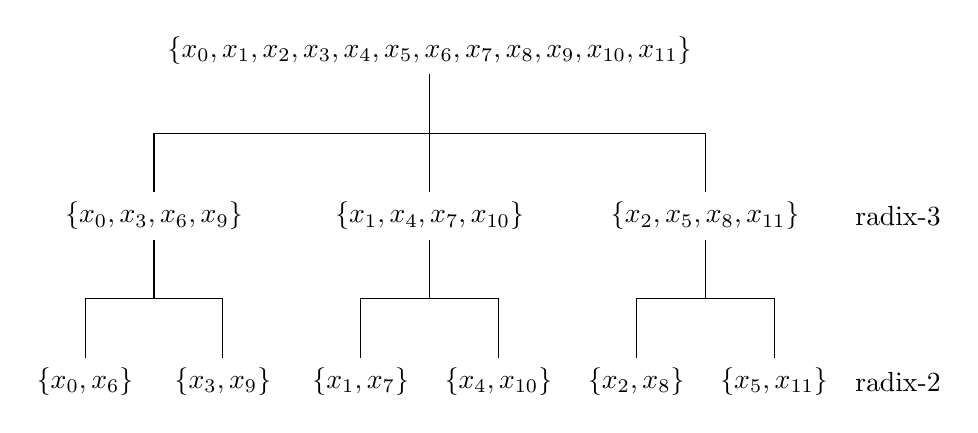
\begin{tikzpicture}[x=3.5cm, y=-1.5cm]
\draw (0, 0) node[anchor=south] {$\{x_0, x_1, x_2, x_3, x_4, x_5, x_6, x_7, x_8, x_9, x_{10}, x_{11}\}$} -- ++(0, 0.5) coordinate
	(j) -| ++(-1, 0.5) node[anchor=north] (r3l) {$\{x_0, x_3, x_6, x_9\}$}
	(j) -- ++( 0, 0.5) node[anchor=north] (r3m) {$\{x_1, x_4, x_7, x_{10}\}$}
	(j) -| ++( 1, 0.5) node[anchor=north] (r3r) {$\{x_2, x_5, x_8, x_{11}\}$}
	(r3l.south) -- ++(0, 0.5) coordinate
		(jl) -| ++(-0.25, 0.5) node[anchor=north]{$\{x_0, x_6\}$}
		(jl) -| ++( 0.25, 0.5) node[anchor=north] {$\{x_3, x_9\}$}
	(r3m.south) -- ++(0, 0.5) coordinate
		(jm) -| ++(-0.25, 0.5) node[anchor=north]{$\{x_1, x_7\}$}
		(jm) -| ++( 0.25, 0.5) node[anchor=north]{$\{x_4, x_{10}\}$}
	(r3r.south) -- ++(0, 0.5) coordinate
		(jr) -| ++(-0.25, 0.5) node[anchor=north]{$\{x_2, x_8\}$}
		(jr) -| ++( 0.25, 0.5) node[anchor=north] (r2r) {$\{x_5, x_{11}\}$};
\node[right=0.1cm of r2r] (r2text) {radix-2};
\node at (r3r -| r2text) {radix-3};
\end{tikzpicture}
\caption{Разложение 12-точечной последовательности}
\label{figure: 12 point decomposition}
\end{figure}

\section{Split-Radix FFT Algorithm}
Объединение radix-2 и radix-4 в результате даёт так называемый \textit{Split-Radix FFT} алгоритм, который имеет ряд преимуществ, включая наименьшее количество умножений/сложений между двумя алгоритмами. Алгоритм основан на наблюдении, что на каждом этапе значение radix-4 лучше для нечетных коэффициентов DFT, а значение radix-2 лучше для четных коэффициентов DFT.

Схему алгоритма можно наблюдать на рисунке \ref{figure: split-radix}.
\begin{figure}[ht]
\centering
%\includegraphics[width=0.9\textwidth]{thesisexample-images/f6}
\begin{tikzpicture}[x=1cm, y=-1cm]
\foreach \x in {0, 1} {
	\edef\xx{\the\numexpr\x * 7}
	\foreach \y in {0, 1, 2, 3} {
		\edef\yy{3.4 * \the\numexpr\y}
		\node[align=center, shape=rectangle, draw, minimum height=3.2cm] (FFT \x\y) at (\xx, \yy) {Четырёх-\\точечный\\DIT FFT};
		\foreach \p in {1, 2, 3, 4}{
			\edef\pp{0.2*\the\numexpr\p}
			\draw ($(FFT \x\y.north west)!\pp!(FFT \x\y.south west)$) -- +(-1, 0) coordinate (FFT \x\y-inp \p);
			\draw ($(FFT \x\y.north east)!\pp!(FFT \x\y.south east)$) -- +( 1, 0) coordinate (FFT \x\y-out \p);
		}
	}
}
\foreach \y in {0, 1, 2, 3}
	\foreach \yy in {0, 1, 2, 3}
		\node [left=1cm of FFT 0\y-inp \the\numexpr\yy+1, anchor=west] {$x_{\the\numexpr\y + \the\numexpr\yy*4}$};
\foreach \y/\d in {0/0, 1/2, 2/1, 3/3}
	\foreach \yy/\dd in {1/0, 2/2, 3/1, 4/3} {
		\node [right=0.1cm of FFT 1\y-out \yy, anchor=west] {$X_{\the\numexpr\d + \the\numexpr\dd*4}^F$};
		\ifnum\d=0\def\dadj{4}\else\edef\dadj{\d}\fi
		\node [below right=0.05cm of FFT 1\y-inp \yy, anchor=north] {\footnotesize{}$W_N^{\the\numexpr(\yy - 1) * \the\numexpr\dadj}$};
	}
\draw[-Latex] (FFT 00-out 1) -- (FFT 10-inp 1);
\draw[-Latex] (FFT 00-out 2) -- (FFT 11-inp 1);
\draw[-Latex] (FFT 00-out 3) -- (FFT 12-inp 1);
\draw[-Latex] (FFT 00-out 4) -- (FFT 13-inp 1);
\draw[-Latex] (FFT 01-out 1) -- (FFT 10-inp 2);
\draw[-Latex] (FFT 02-out 1) -- (FFT 10-inp 3);
\draw[-Latex] (FFT 03-out 1) -- (FFT 10-inp 4);
\end{tikzpicture}
\caption{Упрощённая схема Split-Radix-алгоритма}
\label{figure: split-radix}
\end{figure}

Выше были приведены варианты представления стандартного алгоритма Кули-Туки.
Их можно подробно рассмотреть в \cite{CT-FFT, NTT-using-cyclotomic-polynomials}.
Был рассмотрен весь спектр быстрых radix-алгоритмов, в числе которых БПФ с радиусом 2, 3, 4, разделенным радиусом, DIT и DIF.
Другие быстрые алгоритмы, такие как WFTA, БПФ с простым коэффициентом, UDFHT и т.д. были опущены.

Общей целью этих алгоритмов является значительное снижение вычислительной сложности, ошибок округления/усечения и требований к памяти.
Различные радиусы (radix 2, 3, 4 и т.д.) имеют определенные преимущества перед конкретными платформами, архитектурами и т.д., например, DSP LH9124 – 24-разрядный процессор с фиксированной точкой, который может обрабатывать данные со скоростью до 80 МГц реализован на radix-16 FFT.
Дальнейшее увеличение эффективности БПФ было выполнено в алгоритме Шёнхаге — Штрассена \cite{Schonhage}.

\section{Векторные radix-алгоритмы БПФ}
Аналогично БПФ с радиусом 2, для многомерных сигналов может быть разработан векторно-радиусный двумерный БПФ.
Как и в случае с БПФ radix-2, векторные алгоритмы radix могут быть разработаны как на основе DIT, так и на основе DIF.
Также DIT и DIF могут быть смешаны в одном и том же алгоритме.
На самом деле алгоритмы векторного радиуса существуют для любого радиуса.
В качестве иллюстрации будет рассмотрен векторный радиальный БПФ для двумерного сигнала, основанный на DIT.
Затем легко распространить этот метод на все другие алгоритмы векторного радиуса.
Как и во всех быстрых алгоритмах, преимущества векторного радиального 2-D БПФ заключаются в снижении вычислительной сложности, снижении требований к памяти (хранилищу) и уменьшении ошибок из-за арифметики конечного размера бита.
Векторные алгоритмы radix гораздо более удобны для векторных процессоров.

2D-DFT (и его инверсия) определяется следующим образом:
\begin{equation}\label{eq: 2d fft fwd}\begin{gathered}
X^F(k_1, k_2) = \sum_{n_1=0}^{N_1-1} \sum_{n_2=0}^{N_2-1} x(n_1, n_2) W_{N_1}^{n_1 k_1} W_{N_2}^{n_2 k_2}, \\
k_1 = 0, 1, \dots, N_1 - 1 \text{ и } k_2 = 0, 1, \dots, N_2 - 1.
\end{gathered}\end{equation}
\begin{equation}\label{eq: 2d fft inv}\begin{gathered}
x(n_1, n_2) = \frac{1}{N_1 N_2} \sum_{k_1=0}^{N_1-1} \sum_{k_2=0}^{N_2-1} X^F(k_1, k_2) W_{N_1}^{-n_1 k_1} W_{N_2}^{-n_2 k_2}, \\
n_1 = 0, 1, \dots, N_1 - 1 \text{ и } n_2 = 0, 1, \dots, N_2 - 1.
\end{gathered}\end{equation}

Символически векторный алгоритм radix-2 2-D DIT-FFT может быть представлен образом, представленным на рисунке \ref{figure: 2d vector fft}.
\begin{figure}[ht]
\centering
%\includegraphics[width=0.9\textwidth]{thesisexample-images/f7}
\begin{tikzpicture}[x=3cm, y=-1cm]
\draw (0, 0) node (root) {$(N_1 \times N_2)$-БПФ} +(2, 0) node {$N_1 = 2^{n_1}$, $N_2 = 2^{n_2}$}
	(root.south) -- +(0, 0.5) coordinate (j1);
\foreach \x/\m in {-2/1, -0.7/2, 0.7/3, 2/4}
	\draw (j1) -| +(\x, 0.5) node[anchor=north] (B\m) {$\Big(\frac{N_1}{2}\times\frac{N_2}{2}\Big)$-БПФ};
\draw (B2.south) -- +(0, 0.5) coordinate (j2);
\foreach \x/\m in {-1.3/1, 0/2, 1.3/3, 2.6/4}
	\draw (j2) -| +(\x, 0.5) node[anchor=north] (C\m) {$\Big(\frac{N_1}{4}\times\frac{N_2}{4}\Big)$-БПФ};
\foreach \c/\e/\o in {1/e/e, 2/e/o, 3/o/e, 4/o/o}
	\node [below=0.02cm of C\c.south] {$(\e, \o)$};
\end{tikzpicture}
\caption{Двумерный векторный алгоритм БПФ; здесь $e$ обозначает чётный отсчёт, а $o$ --- нечётный отсчёт}
\label{figure: 2d vector fft}
\end{figure}

При условии равенства $N_1$ и $N_2$ \eqref{eq: 2d fft fwd} раскладывается следующим образом.
\begin{equation*}\begin{aligned}
X^F(k_1, k_2)
 =& \sum_{m_1=0}^{\frac{N}{2}-1}\sum_{m_2=0}^{\frac{N}{2}-1} x(2 m_1, 2 m_2) W_N^{2 m_1 k_1 + 2 m_2 k_2} \\
 &+ \sum_{m_1=0}^{\frac{N}{2}-1}\sum_{m_2=0}^{\frac{N}{2}-1} x(2 m_1 + 1, 2 m_2) W_N^{(2 m_1 + 1) k_1 + 2 m_2 k_2} \\
 &+ \sum_{m_1=0}^{\frac{N}{2}-1}\sum_{m_2=0}^{\frac{N}{2}-1} x(2 m_1, 2 m_2 + 1) W_N^{2 m_1 k_1 + (2 m_2 + 1) k_2} \\
 &+ \sum_{m_1=0}^{\frac{N}{2}-1}\sum_{m_2=0}^{\frac{N}{2}-1} x(2 m_1 + 1, 2 m_2 + 1) W_N^{(2 m_1 + 1) k_1 + (2 m_2 + 1) k_2},
\end{aligned}\end{equation*}
поэтому
\begin{equation}\label{eq: binary fft decomposition}\begin{aligned}
X^F(k_1, k_2)
 =& \Big[\sum_{m_1=0}^{\frac{N}{2}-1}\sum_{m_2=0}^{\frac{N}{2}-1} x(2 m_1, 2 m_2) W_{\frac{N}{2}}^{m_1 k_1 + m_2 k_2}\Big] \\
 &+ W_N^{k_2}\Big[\sum_{m_1=0}^{\frac{N}{2}-1}\sum_{m_2=0}^{\frac{N}{2}-1} x(2 m_1, 2 m_2 + 1) W_{\frac{N}{2}}^{m_1 k_1 + m_2 k_2}\Big] \\
 &+ W_N^{k_1}\Big[\sum_{m_1=0}^{\frac{N}{2}-1}\sum_{m_2=0}^{\frac{N}{2}-1} x(2 m_1 + 1, 2 m_2) W_{\frac{N}{2}}^{m_1 k_1 + m_2 k_2}\Big] \\
 &+ W_N^{k_1+k_2}\Big[\sum_{m_1=0}^{\frac{N}{2}-1}\sum_{m_2=0}^{\frac{N}{2}-1} x(2 m_1 + 1, 2 m_2 + 1) W_{\frac{N}{2}}^{m_1 k_1 + m_2 k_2}\Big].
\end{aligned}\end{equation}
То есть
\begin{equation}\label{eq:fft_recursion}\begin{aligned}
X^F(k_1, k_2) =& S_{00}(k_1,k_2) + S_{01}(k_1, k_2) W_N^{k_2} \\
              +& S_{10}(k_1, k_2) W_N^{k_1} + S_{11}(k_1, k_2) W_N^{k_1 + k_2},
\end{aligned}\end{equation}
причем для всех $i$ и $j$ из $\{0, 1\}$
\begin{equation}\label{eq: fft_recursion_components}\begin{gathered}
S_{i j}(k_1, k_2) = S_{i j}\Big(k_1 + \frac{N}{2}, k_2\Big) = S_{i j}\Big(k_1, k_2 + \frac{N}{2}\Big) \\
= S_{i j}\Big(k_1 + \frac{N}{2}, k_2 + \frac{N}{2}\Big).
\end{gathered}\end{equation}

Поэтому, используя вышеописанные формулы, векторный алгоритм может быть представлен в матричной форме
\begin{equation*}
\begin{bmatrix}
X^F(k_1, k_2) \\
X^F(k_1, k_2 + \frac{N}{2}) \\
X^F(k_1 + \frac{N}{2}, k_2) \\
X^F(k_1 + \frac{N}{2}, k_2 + \frac{N}{2})
\end{bmatrix}
=
\begin{bmatrix}
1 &  1 &  1 &  1 \\
1 & -1 &  1 & -1 \\
1 &  1 & -1 & -1 \\
1 & -1 & -1 &  1
\end{bmatrix}
\begin{bmatrix}
S_{00}(k_1, k_2) \\
W_N^{k_2} S_{01}(k_1, k_2) \\
W_N^{k_1} S_{10}(k_1, k_2) \\
W_N^{k_1 + k_2} S_{11}(k_1, k_2)
\end{bmatrix},
\end{equation*}
где $k_1, k_2 \in \mathbb{Z}_{\frac{N}{2}}$.

Это матричное отношение может быть представлено в виде графа, представленного на рисунке \ref{fig: fft 2d butterfly}.
\begin{figure}[ht]
\centering
%\includegraphics[width=0.9\textwidth]{thesisexample-images/f9}
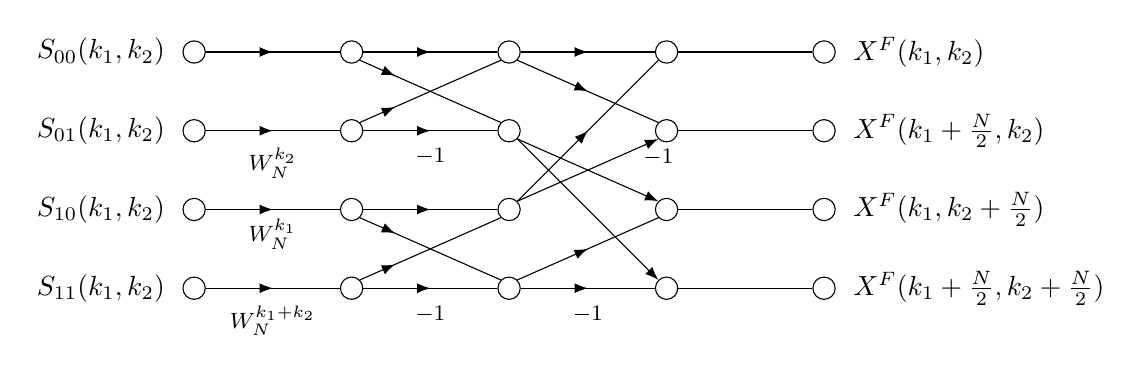
\begin{tikzpicture}[x=2cm,y=-1cm,midarr/.style={postaction=decorate, decoration={markings, mark=at position 0.5 with \arrow{Latex}}},quadarr/.style={postaction=decorate, decoration={markings, mark=at position 0.25 with \arrow{Latex}}}]
\foreach \y in {0, 1, 2, 3}
	\foreach \x in {0, 1, 2, 3, 4}
		\node[shape=circle, inner sep=0.1cm, draw] (n\x\y) at(\x, \y) {};
\node[left=0.1cm of n00] {$S_{00}(k_1, k_2)$}; \node[right=0.1cm of n40] {$X^F(k_1, k_2)$};
\node[left=0.1cm of n01] {$S_{01}(k_1, k_2)$}; \node[right=0.1cm of n41] {$X^F(k_1 + \frac{N}{2}, k_2)$};
\node[left=0.1cm of n02] {$S_{10}(k_1, k_2)$}; \node[right=0.1cm of n42] {$X^F(k_1, k_2 + \frac{N}{2})$};
\node[left=0.1cm of n03] {$S_{11}(k_1, k_2)$}; \node[right=0.1cm of n43] {$X^F(k_1 + \frac{N}{2}, k_2 + \frac{N}{2})$};
\draw[midarr](n00.east) -- (n10.west); \draw[midarr](n10.east) -- (n20.west); \draw[midarr](n20.east) -- (n30.west); \draw(n30.east) -- (n40.west); \draw[quadarr](n10.south east) -- (n21.north west); \draw[midarr] (n20.south east) -- (n31.north west);
\draw[midarr](n01.east) -- node[below=0.1cm,font=\footnotesize]{$W_N^{k_2}$} (n11.west); \draw[midarr](n11.east) -- node[below=0.1cm,font=\footnotesize]{$-1$} (n21.west); \draw (n31.east) -- (n41.west); \draw[quadarr] (n11.north east) -- (n20.south west); \draw[-Latex] (n21.south east) -- (n32.north west); \draw[-Latex] (n21.south east) -- (n33.north west);
\draw[midarr](n02.east) -- node[below,font=\footnotesize]{$W_N^{k_1}$} (n12.west); \draw[midarr] (n12.east) -- (n22.west); \draw (n32.east) -- (n42.west); \draw[quadarr] (n12.south east) -- (n23.north west); \draw[midarr] (n22.north east) -- (n30.south west); \draw[-Latex] (n22.north east) -- node[at end, below, font=\footnotesize] {$-1$} (n31.south west);
\draw[midarr](n03.east) -- node[below=0.1cm, font=\footnotesize] {$W_N^{k_1 + k_2}$} (n13.west); \draw[midarr](n13.east) -- node[below=0.1cm, font=\footnotesize] {$-1$} (n23.west); \draw[midarr](n23.east) -- node[below=0.1cm, font=\footnotesize] {$-1$} (n33.west); \draw(n33.east) -- (n43.west); \draw[quadarr] (n13.north east) -- (n22.south west); \draw[midarr](n23.north east) -- (n32.south west);
\end{tikzpicture}
\caption{Граф векторного алгоритма 2-D DIT-DFT для $N1 = N2 = 4$}
\label{fig: fft 2d butterfly}
\end{figure}
Децимация выполняется $\log_2 N$ раз.
Каждый шаг децимации включает в себя $N^2/4$ бабочек.
Для каждой бабочки нужно три комплексных умножения и восемь комплексных сложений.
\section{Алгоритм Шёнхаге-Штрассена}
Алгоритм использует рекурсивные быстрые преобразования Фурье в кольцах с $2n + 1$ элементами.

При данных входных числах $x$ и $y$ и целого $N$, алгоритм вычисляет произведение $xy \pmod{2^N + 1}$.
При условии, что $N$ достаточно велико, это просто произведение.

Каждое входное число разделяется на векторы $X$ и $Y$ по $2^k$ частей каждый, где $2^k$ делит $N$.

Вычисляется произведение $X$ и $Y$ по модулю $2^N + 1$, используя негациклическую свертку.

Затем выполняется перенос по модулю $2^N  + 1$, и получается финальный результат. Более подробный разбор алгоритма будет приведён в главе 2.


\chapter{Проектирование алгоритмов дискретного и быстрого теоретико-числовых преобразований для быстрого решения задач расчета свертки в целых числах и длинного умножения}
В данной главе рассмотрено представление алгоритма теоретико-числового преобразования и зафиксированы его отличительные особенности.

Были обоснованы критерии выбора модуля и примитивного корня алгоритма.
По установленным критериям с помощью программного обеспечения были подобраны эти величины.

Были указаны особенности использования 512-разрядных расширений 256-разрядных инструкций Advanced Vector Extensions (AVX-512) SIMD для архитектуры набора инструкций x86.

Была описана процедура формирования спектров входных сигналов.
\section{Описание алгоритма теоретико-числового преобразования}
В данной работе используется приближенная форма преобразования Фурье –-- теоретико-числовое преобразование \cite{NTT-Lattice}.

Теоретико-числовые преобразования (ТЧП) были разработаны в начале семидесятых годов на основе теории чисел.
Они представляют собой дискретные преобразования Фурье, определенные над конечными полями и кольцами --- поскольку эти преобразования выполняются по арифметическому модулю --- по модулю простого числа, они проявляют много интересных свойств, которые полезны для цифровой обработки сигналов.
ТЧП вычисляются в целочисленной области, и, следовательно, они считаются превосходящими по сравнению с уже существующими БПФ.

Традиционные теоретико-числовые преобразования, которые, избегая арифметики с плавающей точкой, обеспечивают точные целочисленные свертки, могут быть заданы взвешенными встречными частями \cite{FFT-convolutions}.
Пусть целые числа, $x$ и $y$, выражены в сбалансированных представлениях типа \eqref{eq: number_polynomial}
\begin{equation}\label{eq: number_polynomial}
x = \sum_{j=0}^{N-1} x_j W^j,
\end{equation}
где $0 \leq x_j < W$.

Тогда циклические и негациклические свертки удовлетворяют неравенству \eqref{eq: convolution_upper_bound}
\begin{equation}\label{eq: convolution_upper_bound}
\big\vert(x *^a y)_n\big\vert \leq \frac{N W^2}{4},
\end{equation}
где операция "$*^a$" осуществляет взвешенную свёртку для каждого $n\in\mathbb{Z}_N$ \cite{FFT-convolutions}.

Рассматривается теоретико-числовые взвешенные преобразования, основанные на арифметике над конечным коммутативным ассоциативным кольцом с единицей.
Практическим частным случаем является:
\begin{equation}\label{eq: ntt}
X_k = \sum_{j=0}^{N-1} x_j A^j g^{-j k} \in R,
\end{equation}
\begin{whereblock}
	$A$ --- обратимый в поле $R$ весовой коэффициент, который можно принять равным 1 для циклического случая, и равным $-1$ --- для негациклического (значение $A=-1$ является примитивным корнем степени $2 N$ из единицы в $R$);\\
	$g$ --- примитивный корень степени $N$ из единицы в $R$.
\end{whereblock}

Для циклического случая можно принять $A=1$, для негациклического случая --- $A=-1$ --- примитивный корень из единицы степени $2 N$ в $R$.

В негациклическом случае достаточно использовать $g = A^2$.
Когда используется конечное поле $R=GF(p)$ для простого числа $p$, вследствие \eqref{eq: convolution_upper_bound} достаточно, чтобы выполнялось неравенство
\begin{equation}\label{eq: schonhage_strassen field limit}
\frac{N W^2}{4} < \frac{p}{2}.
\end{equation}
Затем взвешенные преобразования типа \eqref{eq: ntt} со всей арифметикой, выполненной по модулю $p$, могут быть использованы для однозначного определения (возможно, биполярных) элементов преобразования \cite{loop-ntt}.
Могут быть получены границы, более четкие, чем \eqref{eq: schonhage_strassen field limit}, особенно если учитывать заполнение старших цифр нулями или специальные симметрии.
Популярным выбором является выбор чисел Ферма $p = F_m = 2^{2^m} + 1$.
Результирующее преобразование числа Ферма (FNT) обладает привлекательными свойствами \cite{ArithmeticsForFNT}, но имеет один существенный недостаток.
Преимущества FNT заключаются в способности выполнять \eqref{eq: ntt} (с генерированием скаляра $A$, равного степени 2) только на основе операций сдвига и сложения, в то время как недостаток заключается в том, что максимально допустимые длины выполнения FNT довольно ограничены.

Пример FNT может быть представлен следующим образом.
Изначально $W = 2^{16}$, и $N = 64$‚ так что циклическая или негациклическая свертка желательна для произведения $x$ и $y$ из $\mathbb{Z}_{W^N}$.
Каждый из множителей имеет размер не более 1024 бит.
Поскольку $N W^2  = 2^{38}$‚ достаточно по \eqref{eq: schonhage_strassen field limit} выбрать $p=F_6=2^64+1$.
Выбирается $A = 2$, который является 64-м корнем из $-1 \pmod{F_6}$, и $g = 4$.
Тогда взвешенное преобразование
\begin{equation}\label{eq: ntt example}
X_k = \sum_{j=0}^{63} x_j 2^j 4^{-jk} \pmod{F_6}
\end{equation}
может использоваться для вычисления негациклических сверток, соответствующих исходным целым числам $x$ и $y$, имеющим размер не более 1024 бит каждый.
Очевидно, что \eqref{eq: ntt example} или его еще более простой циклический аналог могут быть выполнены с помощью операций сдвига, сложения и операций с модулем Ферма без какого-либо явного требуемого умножения.
Из-за ограничений на длину при кодировании поворотов FNT становится сложно выполнять точное умножение целых чисел, содержащих, сотни тысяч битов \cite{ArithmeticWithNTT, NT-in-DSP}.
Эту проблему помогают решить различные многомерные подходы или преобразование Галуа \cite{FFT-over-FF}, для которого выражения, такие как \eqref{eq: ntt}, должны быть вычислены в $GF(p^2)$, где $p = 2^q - 1$ --- простое число Мерсенна.
Эти преобразования используют два факта.

Во-первых, для арифметики в $GF(p^2)$ предполагается, что каждый элемент поля равен $a + bi$, при этом все действительные и мнимые компоненты подвергаются редукции по модулю $p$ на каждом этапе.
Во-вторых, порядок мультипликативной группы равен $p^2-1=(p+1)(p-1)$, который делится на $2^{q + 1}$, что позволяет на практике использовать достаточный период, равный степени двух.

Пусть $h$ --- примитивный мультипликативный $2^{q + 1}$-й корень из 1 в $GF(p^2)$.
Для $r \leq q$
\begin{equation}\label{eq: simplifying ntt 1}
N = 2^r,\quad A=h^{(p-1) 2^{q-r-1}}, \quad g=A^2.
\end{equation}

Поскольку $A^N = -1$, в соответствии с ограничением \eqref{eq: schonhage_strassen field limit} может выполняться циклическая свертка длиной $N$ (где $A$ просто исключено из \eqref{eq: ntt}) или свертка с отрицательными цифрами.
Если $r$ строго меньше $q$, то выбираются
\begin{equation}\label{eq: simplifying ntt 2}
N = 2^r,\quad A=h^{(p-1) 2^{q-r-2}}, \quad g=A^4.
\end{equation}

По теореме Крейцбурга и Таше можно получить выражения замкнутой формы для примитивных корней в $GF(p^2)$.
Например,
$$
h = 2^{2 q - 2} + (-3)^{2 q - 2}i
$$
всегда является примитивным мультипликативным $2^{q + 1}$-ым корнем из 1.
Из \eqref{eq: simplifying ntt 1} следует, что можно использовать периоды от двух до $2^q$ для циклической или негациклической свертки.

Дальнейшим наблюдением является то, что $g \cdot g^*=1 \bmod{p}$, так что вышеупомянутые методы преобразования реального сигнала и реального результата могут быть применены, к взвешенным случаям \eqref{eq: ntt} с учетом соответствующих симметрий $X$.

Полезный пример приложений преобразования Галуа возникает, когда $p$ является простым числом Мерсенна $2^{61} - 1$.
Для фиксированной базы $W = 2^{16}$ можно, в силу \eqref{eq: schonhage_strassen field limit}, рассмотреть периоды до размера $M = 2^{27}$ цифр.
Программы для взвешенной свертки могут быть реализованы, начиная с одного примитивного корня, такого как
$$
h = 2137483648+1033321771269002680 i.
$$

Затем используются соотношения \eqref{eq: simplifying ntt 1} или \eqref{eq: simplifying ntt 2} для обработки определенных длин $2^r$.
Например, для умножения двух целых чисел, каждое из которых имеет не более 1 миллиона бит.
Можно продолжить с прямоугольными свертками следующим образом.
В соответствии с \eqref{eq: simplifying ntt 2}, делается выбор:
\begin{gather*}
N = 2^{16}, \\
A = h^{(p-1)\cdot 2^{43}} = 1973234539278172120+1244201103777839971 i, \\
g = A^4 = 1510466207055935382+120042544849731353i,
\end{gather*}
для которого можно проверить, что $A^N = i$, следовательно, $g^N = 1$ в $GF(p^2)$.
Тогда \eqref{eq: ntt} и взвешенную формулу свертки можно использовать для вычисления $n$-го разряда произведения как $\Re\big((x *^a y)_n\big)$ для $n < N$, и $\Im\big((x *^a y)_{n-N}\big)$ для $n \geq N$.
Хотя в этом примере требуются сложные БПФ с умножением с высокой 64-х битной точностью‚ \eqref{eq: schonhage_strassen field limit} гарантирует, что умножение является точным, без ошибок, связанных с вычислениями с плавающей точкой.
\section{Отличие теоретико-числового преобразования от более стандартных БПФ-алгоритмов}
ТЧП сигнала выполняется в целочисленной области, тогда как DFT/FFT – в комплексной области.
Коэффициенты NTT не имеют никакого физического смысла, поскольку операции выполняются по арифметическому модулю.
Из-за модульной арифметики все выходные данные являются целыми числами в конечном кольце, заданным модулем, и никаких приближений не происходит.
Следовательно, ТЧП не имеют ошибок округления, как в стандартных алгоритмах.
В частном случае, когда реализуется представление длинных данных в виде скаляров $x_i$ в \eqref{eq: number_polynomial}, умножение на степени W осуществляется операциями посимвольного сдвига, то есть битового сдвига в двоичном представлении $X$ в \eqref{eq: number_polynomial}.
В этом случае в ТЧП, все умножения могут быть преобразованы в сдвиги и сложения.
Это намного проще, чем сложные умножения произвольных действительных, и тем более комплексных чисел \cite{fast-multiplication-long-ints}; следовательно, FNT быстрее, чем FFT.

Если две последовательности $x(n)$ и $h(n)$ имеют битовые представления $b_1$ и $b_2$, а длина преобразования равна $N$, то вывод свертки $y(n)$ имеет максимальное $b_1+b_2+\log_2 ⁡N$ битовое представление.
В БПФ каждая выборка данных имеет действительную и мнимую части, для этого требуется два слова, одно для действительного и одно для мнимого.
Следовательно, требования к хранилищу и оборудованию как для NTT, так и для FFT остаются практически одинаковыми.

В методе FNT умножение на степень 2 реализуется как операции сдвига и сложения битов, которые намного проще по сравнению со сложными умножениями, требуемыми в методе DFT \cite{RingLWE-multiplication}.
Это обеспечивает значительную экономию времени вычислений и, следовательно, алгоритмы NTT работают быстрее, чем FFT.

\section{Программная реализация}
Согласно заданию, вышеописанный алгоритм необходимо представить в векторной форме.
Возможность векторной реализации вычислений представлена во многих современных процессорах, в данной работе для проектирования реализации, использующей AVX-512, использован эмулятор Intel\textregistered{} Software Development Emulator (Intel SDR), а для экспериментальных измерений, результаты которых представлены в главе \ref{chapter: experiments}, --– микропроцессор Intel Core i9-10980XE, реализующий архитектуру CascadeLake AVX-512 –-- это 512-разрядные расширения 256-разрядных инструкций Advanced Vector Extensions SIMD для архитектуры набора инструкций x86 (ISA), предложенных Intel в июле 2013 года и реализованных в процессорах Intel Xeon Phi x200 и Skylake-X; это включает Core-X серии (исключая Core i5-7640X и Core i7-7740X), а также новое семейство масштабируемых процессоров Xeon и встроенную серию Xeon D-2100.

Сначала выполняется подбор модуля используемого кольца.
В стандартном алгоритме Шёнхаге-Штрассена используется $m=2^{64}+1$.
Однако, в данной работе такой модуль не подходит, так как нет векторных регистров, использующих скаляры из $\mathbb{Z}_{2^{128}}$. Значение $m=2^{64}-1$ так же не подходит, так как в кольце $\mathbb{Z}_{2^{64}-1}$ нет принципиального корня 16-й степени из единицы.
Также не подходит значение $m = 2^{64}$, так как в $\mathbb{Z}_{2^{64}}$ не существует мультипликативной инверсии 16, умножение на которую требуется при обратном теоретико-числовом преобразовании, поскольку $\gcd⁡(16, 2^{64}) \ne 1$.

Таким образом, был выполнен перебор возможных $m$, начиная с $2^{64}-1$, и осуществлён произвольный выбор тех из них, которые одновременно удовлетворяют следующим критериям:
\begin{enumerate}
\item $\gcd(m, 16) = 1$,
\item $\lambda(m) \bmod{16} = 0$, где $\lambda(m)$ --- это функция Кармайкла,
\item $\exists a\bigg[a \in \mathbb{Z}_m \land a^{\lambda(m)} = 1 \land \gcd\Big(a^\frac{\lambda(m)}{16} - 1, m\Big) = 1\bigg]$.
\end{enumerate}

Расчёт функции Кармайкла выполняется следующим образом:
$$
\lambda(m)=
\begin{cases}
&\varphi(m), \text{ если } m \in \big\{p^n \mid p \in \mathcal{P} \land n \in \mathbb{N} \land (p \ge 3 \lor n < 2)\big\}, \\
&\frac{\varphi(m)}{2}, \text{ если } m \in \{2^n \mid n \in \mathbb{N} \land n \ge 3\}, \\
&\operatorname{lcm}_{i=1}^q\big(\lambda(p_i^{k_i})\big), \text{ если } m \in \begin{aligned}[t]\Big\{\prod_{i=1}^q p_i^{k_i} \mid &p_i\in\mathcal{P} \land k_i\in\mathbb{N} \land q \geq 2\\
&\land i \ne j \implies p_i \ne p_j\Big\},\end{aligned}
\end{cases}
$$
\begin{whereblock}
$\varphi(m)$ --- тотиента Эйлера,\\
$\mathcal{P}$ --- множество всех простых чисел.
\end{whereblock}

В третьем случае значение функции рассчитывается рекуррентно как наименьшее общее кратное (lcm --– least common multiplier) значений функции Кармайкла всех простых множителей ($p_i$ в соответствующей степени $k_i$) в разложении числа $m$, $q$ –-- число уникальных простых множителей в разложении $m$.
Для размеров $m$, рассматриваемых в рамках настоящей работы, разложение числа $m$ на простые достаточно выполнить путем проверки делимости на малые простые, доступные, например, в \cite{IrregularPrimes, crandallprimes}.

Значение функции Кармайкла --– минимальное целое такое, что
$$
\forall a\big[a \in \mathbb{Z}_m \implies a^{\lambda(m)} = 1 \bmod{m}\big].
$$

Тотиента Эйлера вычисляется по формуле
$$
\varphi(m) = \prod_{i=1}^q p_i^{k_i - 1} (p_i - 1).
$$

Далее, найдя $m$, значение примитивного корня 16-й степени принимается равным тому значению $g=a^\frac{\lambda(m)}{16}$ в третьем критерии, для которого справедливо
$$
\forall n\big[n\in\mathbb{N} \land n < 16 \implies g^n \ne 1 \bmod{m}\big].
$$

В настоящей работе  использованы следующие найденные значения $m$ и $g$:
\begin{align*}
m &= \textrm{0xffffffffffffffa1}, \\
g &= \textrm{0xe97df2aaae3ae452},
\end{align*}
где "0x" означает представление в шестнадцатеричной системе счисления.

Далее, выполняется ввод двух входящих потоков данных.
Входные данные умещаются в один "период", под которым понимается набор из 16 элементов данных, формируются целочисленные (определенные над кольцом $\mathbb{Z}_m$) спектры этих сигналов.
Далее по спектрам восстанавливается информация и сравнивается с вошедшим потоком данных. В случае совпадения выполняется умножение спектров.


\chapter{Векторизация быстрого теоретико-числового преобразования и длинного умножения}\label{chapter: implementation}
В данной главе рассмотрены методы и аспекты векторной реализации целочисленной арифметики.
Рассмотрена структура векторного регистра, особенности реализации векторной арифметики \cite{IntelManual, ArmManual}.

Предложен алгоритм векторного умножения чисел из множества $\mathbb{Z}_{2^{512}}$, представленных векторами из изоморфного множества $\mathbb{Z}_{2^{16}}^8$, которое реализуется векторным расширением AVX-512.

\section{Основные аспекты векторизации вычислений}
Векторизация вычислений заключается в принципе выполнения нескольких однотипных операций над множественным потоком данных.
Этот принцип также называют SIMD –-- single instruction, multiple data.
Использование векторных инструкций, как правило, положительно сказывается на производительности вычислений.

Векторные вычисления реализуются как в специализированных процессорах, так и с помощью векторных расширений.
В данной работе используется векторное расширение AVX-512, имеющее 32 векторных регистра длиной 512 бит, которые называются ZMM0\dots ZMM15.

\section{Реализация умножения в $\mathbb{Z}_{2^{60}}$ средствами AVX-512}
По заданию данный алгоритм необходимо ускорить путём векторного представления. Это выполнено с помощью набора векторных инструкций AVX-512 для процессоров Intel серии Core-X.

Сначала входящие сигналы длиной 64 бита каждый разделяются на два 32-битовых символа, разделяясь на старший и младший символ, это изображено на блок-схеме на рисунке \ref{eq: vector operands example}.
\begin{figure}[ht]
\centering
%\includegraphics[width=0.7\textwidth]{thesisexample-images/f10}
\begin{tikzpicture}[every node/.style={draw}, header/.style={draw=none}]
\foreach \c\v/\V in {0/x/X, 6/y/Y} {
	\node (\v h) at (\c,0) {$\v_{hi}$ (32 бит)};
	\node[right=0 of \v h.east, anchor=west] (\v l) {$\v_{lo}$ (32 бит)};
	\node[header, above=0.1cm of \v h.north east] {$\V$ (64 бит)};
}
\end{tikzpicture}
\caption{Разложение входящих 64-битовых потоков данных на два 32-битовых разряда}
\label{eq: vector operands example}
\end{figure}

Далее выполняется операция, графически представленная на рисунке \ref{eq: vector vertical operation example}.
\begin{figure}[ht]
\centering
%\includegraphics[height=6em]{thesisexample-images/f11}
\begin{tikzpicture}[x=2cm, y=-1.5cm]
\foreach \v/\y in {x/0, y/1} {
	\node[draw] (\v hi) at (0, \y) {$\v_{hi}$ (32 бит)};
	\node[draw, right=0cm of \v hi.east, anchor=west] (\v lo) {$\v_{lo}$ (32 бит)};
}
\foreach \p in {hi, lo} {
	\draw (x\p.south) -- (y\p.north);
	\node[fill=white, inner sep=0] at ($(x\p.south)!0.5!(y\p.north)$) {$\times$};
	\path (y\p.south) +(0, 0.1) [draw, ->] -- +(0, 0.3) coordinate(out\p);
	\node[below=-0.05 of out\p, anchor=north] {$p_{\p}$};
}
\end{tikzpicture}
\caption{Умножение старших и младших символов изначально принятых значений}
\label{eq: vector vertical operation example}
\end{figure}

Полученные значения сдвигаются в область ещё более старших и младших разрядов, проверяются на не превышение значения модуля и суммируются, образуя одно 64-битовое слово
$$
p = p_{hi} + p_{lo},
$$
которое, в свою очередь, проверяется на переполнение.
Проверка выполняется путем сравнения суммы с одним из слагаемых, то есть переполнение возникает при $p_{hi}+p_{lo} < p_{hi}$  или $p_{hi}+p_{lo} < p_{lo}$.

Программная реализация представлена на рисунке \ref{fig: avx512 32 bit multiplication}.
\begin{figure}[ht]
\centering
%\includegraphics[width=\textwidth]{thesisexample-images/f12}
\begin{lstlisting}[language=C]
__m512i p_hi = _mm512_mul_epu32(x_hi, y_hi);
__m512i p_lo = _mm512_mul_epu32(x_lo, y_lo);
__m512i p_hi_hi = _mm512_srli_epi64(p_hi, 32);
__m512i p_hi_lo = _mm512_mask_mov_epi32(p_hi, lo_msk, p_hi);
__m512i p;
p_hi_hi = _mm512_mul_epu32(p_hi_hi, epi64_mod);
p_hi_lo = _mm512_mul_epu32(p_hi_lo, epi64_mod);
p_hi_lo = _mm512_add_epi64(p_hi_lo,
       _mm512_slli_epi64(p_hi_hi, 32));
p_hi_hi = _mm512_mul_epu32(_mm512_srli_epi64(p_hi_hi, 32),
	epi64_mod);
p_hi = _mm512_add_epi64(p_hi_lo, p_hi_hi);
p = _mm512_add_epi64(p_hi, p_lo);
p = _mm512_mask_sub_epi64(p,
       _mm512_cmp_epu64_mask(p, p_hi, _MM_CMPINT_LT /*1*/), p, m);
\end{lstlisting}
\caption{Умножение старших и младших разрядов, сдвиг результатов в нужную область, их сумма и проверка на переполнение}
\label{fig: avx512 32 bit multiplication}
\end{figure}

Заметим, что сложение можно реализовать путём выражения суммы в избыточной системе счисления.
Это позволяет выполнять сложение без взаимосвязи между разрядами \cite{ChusovLychev}.

Далее выполняется перекрёстное умножение разрядов --- старший на младший.
Два полученных 32-битовых значения также суммируются (рис.~\ref{fig: vector cross-lane multiplication}) и проверяются на переполнение заданного максимального объёма в 64 бита.
\begin{figure}[ht]
\centering
%\includegraphics[height=6em]{thesisexample-images/f13}
\begin{tikzpicture}[x=2cm, y=-1.5cm]
\foreach \v/\y in {x/0, y/1} {
	\node[draw] (\v hi) at (0, \y) {$\v_{hi}$ (32 бит)};
	\node[draw, right=0cm of \v hi.east, anchor=west] (\v lo) {$\v_{lo}$ (32 бит)};
}
\foreach \v/\p/\vl in {x/south/y, y/north/x} {
	\foreach \vv/\ppb/\ppe in {hi/east/west,lo/west/east} {
		\coordinate (\v\vv p) at ($(\v\vv.\p\space\ppb)!0.2!(\v\vv.\p\space\ppe)$);}
}
\foreach \v/\vl in {x/y, y/x}
	\draw (\v hip) -- (\vl lop);
\node[fill=white, inner sep=0.05] at($(xhip)!0.5!(ylop)$) {$\times$};
\node[fill=white, draw, below=-0.2 of yhi.south east, anchor=north] (hadd) {$+$};
\draw (yhi.south) +(0, 0.1) [->] |- (hadd.west);
\draw (ylo.south) +(0, 0.1) [->] |- (hadd.east);
\draw (hadd.south) +(0, 0.1) [->] -- +(0, 0.4) coordinate (output);
\node[below=-0.05 of output, anchor=north] {$p_m$};
\end{tikzpicture}
\caption{Умножение старших и младших разрядов $p_m = x_{hi} y_{lo} + x_{lo} y_{hi}$}
\label{fig: vector horizontal operation example}
\end{figure}
Результаты умножений вновь суммируются и проверяются на переполнение.
Программная реализация представлена на рисунке \ref{fig: vector cross-lane multiplication}.
\begin{figure}[ht]
\centering
%\includegraphics[width=\textwidth]{thesisexample-images/f14}
\begin{lstlisting}[language=C]
__m512i p_m;
x_hi = _mm512_mul_epu32(x_hi, y_lo);
y_hi = _mm512_mul_epu32(y_hi, x_lo);
p_m = _mm512_add_epi64(x_hi, y_hi);
p_m = _mm512_mask_sub_epi64(p_m,
         _mm512_cmp_epu64_mask(p_m, y_hi, _MM_CMPINT_LT /*1*/),
         p_m, m);
p_hi = _mm512_srli_epi64(p_m, 32);
p_hi = _mm512_mul_epu32(p_hi, epi64_mod);
p_lo = _mm512_slli_epi64(p_m, 32);
p_m = _mm512_add_epi64(p_lo, p_hi);
p_m = _mm512_mask_sub_epi64(p_m,
         _mm512_cmp_epu64_mask(p_m, p_lo, _MM_CMPINT_LT /*1*/),
         p, m);
p = _mm512_add_epi64(p, p_m);
p = _mm512_mask_sub_epi64(p,
         _mm512_cmp_epu64_mask(p, p_m, _MM_CMPINT_LT /*1*/), p, m);
p = _mm512_mask_sub_epi64(p,
         _mm512_cmp_epu64_mask(p, m, _MM_CMPINT_NLT /*5*/), p, m);
\end{lstlisting}
\caption{Перекрёстное умножение старших и младших разрядов, сдвиг результатов в нужную область, их сумма и проверка на переполнение}
\label{fig: vector cross-lane multiplication}
\end{figure}

\section{Реализация ДПФ с помощью AVX-512}
Для выполнения ДПФ вошедшие данные представляются в виде матрицы, над которой выполняется быстрое преобразование Фурье и, следом, обратное преобразование Фурье.
Их программное представление можно наблюдать на рисунке \ref{fig: avx512 nnt}.
\begin{figure}[ht]
\centering
%\includegraphics[width=\textwidth]{thesisexample-images/f15}
\begin{lstlisting}[language=C]
static void my_mm512_fft_epi64x2(
         __m512i time_lo, __m512i time_hi,
	 __m512i* spec_lo, __m512i* spec_hi) {
         my_mm512_fft_epi64x2_custom_matrix(
                  time_lo, time_hi, spec_lo, spec_hi,
                  fft_matrix.fwd_powers);
}
static void my_mm512_ifft_epi64x2(__m512i spec_lo, __m512i spec_hi,
         __m512i* time_lo, __m512i* time_hi) {
         __m512i h, l, r;
         my_mm512_fft_epi64x2_custom_matrix(spec_lo, spec_hi, &l, &h,
                  fft_matrix.bwd_powers);
         r = _mm512_set1_epi64(reciprocal(UINT64_C(16), modulo));
         *time_lo = my_mm512_mul_epi64_mod(l, r);
         *time_hi = my_mm512_mul_epi64_mod(h, r);
}
void fnt_avx512_16(const unsigned long long* time,
 unsigned long long* spectrum) {
         __m512i hi, lo;
         my_mm512_fft_epi64x2(
                  _mm512_loadu_si512(time),
                  _mm512_loadu_si512(&time[8]),
                  &lo, &hi);
         _mm512_storeu_si512(spectrum, lo);
         _mm512_storeu_si512(&spectrum[8], hi);
}
void ifnt_avx512_16(const unsigned long long* spectrum,
         unsigned long long* time) {
         __m512i hi, lo;
         my_mm512_ifft_epi64x2(
                  _mm512_loadu_si512(spectrum),
                  _mm512_loadu_si512(&spectrum[8]),
                  &lo, &hi);
         _mm512_storeu_si512(time, lo);
         _mm512_storeu_si512(&time[8], hi);
}
\end{lstlisting}
\caption{Прямое и обратное ДПФ с использованием инструкций AVX-512 для векторов и масок}
\label{fig: avx512 nnt}
\end{figure}

Полученная матрица поворота умножается, в реализации \verb+my_mm512_fft_epi64x2_custom_matrix+, на вектор данных, обозначающих временную область сигнала в случае прямого преобразования Фурье и на вектор данных обозначающих спектр сигнала в случае обратного преобразования Фурье.
При этом матрица 16x16 разделяется надвое, по восемь столбцов в каждой части.
Все умножения выполняются по модулю.
В случае прямого ДПФ:
$$
\begin{pmatrix}
W_{LT} & W_{RT} \\
W_{LB} & W_{RB}
\end{pmatrix}
\cdot
\begin{pmatrix}
T_L \\
T_B
\end{pmatrix},
$$
где $W$ –-- фрагмент матрицы поворота, $T$ –-- фрагмент значений временной области сигнала.

В случае обратного ДПФ:
$$
\begin{pmatrix}
W_{LT} & W_{RT} \\
W_{LB} & W_{RB}
\end{pmatrix}
\cdot
\begin{pmatrix}
S_L \\
S_B
\end{pmatrix}.
$$

При этом, собираемые матрицы имеют вид:
$$
W_{LT} =
\begin{bmatrix}
W^0 &   W^0  &   W^0  &   W^0  &   W^0  &   W^0  &   W^0  &   W^0  \\
W^0 &   W^1  &   W^2  &   W^3  &   W^4  &   W^5  &   W^6  &   W^7  \\
W^0 &   W^2  &   W^4  &   W^6  &   W^8  & W^{10} & W^{12} & W^{14} \\
W^0 &   W^3  &   W^6  &   W^9  & W^{12} & W^{15} &   W^2  &   W^5  \\
W^0 &   W^4  &   W^8  & W^{12} &   W^0  &   W^4  &   W^8  & W^{12} \\
W^0 &   W^5  & W^{10} & W^{15} &   W^4  &   W^9  & W^{14} &   W^3  \\
W^0 &   W^6  & W^{12} &   W^2  &   W^8  & W^{14} &   W^4  & W^{10} \\
W^0 &   W^7  & W^{14} &   W^5  & W^{12} &   W^3  & W^{10} &   W^1  \\
\end{bmatrix},
$$
$$
W_{LB} =
\begin{bmatrix}
W^0 &   W^8  &   W^0  &   W^8  &   W^0  &   W^8  &   W^0  &   W^8  \\
W^0 &   W^9  &   W^2  & W^{11} &   W^4  & W^{13} &   W^6  & W^{15} \\
W^0 & W^{10} &   W^4  & W^{14} &   W^8  &   W^2  & W^{12} &   W^6  \\
W^0 & W^{11} &   W^6  &   W^1  & W^{12} &   W^7  &   W^2  & W^{13} \\
W^0 & W^{12} &   W^8  &   W^4  &   W^0  & W^{12} &   W^8  &   W^4  \\
W^0 & W^{13} & W^{10} &   W^7  &   W^4  &   W^1  & W^{14} & W^{11} \\
W^0 & W^{14} & W^{12} & W^{10} &   W^8  &   W^6  &   W^4  &   W^2  \\
W^0 & W^{15} & W^{14} & W^{13} & W^{12} & W^{11} & W^{10} &   W^9
\end{bmatrix},
$$
$$
W_{RT} =
\begin{bmatrix}
W^0 &   W^0  &   W^0  &   W^0  &   W^0  &   W^0  &   W^0  &   W^0  \\
W^8 &   W^9  & W^{10} & W^{11} & W^{12} & W^{13} & W^{14} & W^{15} \\
W^0 &   W^2  &   W^4  &   W^6  &   W^8  & W^{10} & W^{12} & W^{14} \\
W^8 & W^{11} & W^{14} &   W^1  &   W^4  &   W^7  & W^{10} & W^{13} \\
W^0 &   W^4  &   W^8  & W^{12} &   W^0  &   W^4  &   W^8  & W^{12} \\
W^8 & W^{13} &   W^2  &   W^7  & W^{12} &   W^1  &   W^6  & W^{11} \\
W^0 &   W^6  & W^{12} &   W^2  &   W^8  & W^{14} &   W^4  & W^{10} \\
W^8 & W^{15} &   W^6  & W^{13} &   W^4  & W^{11} &   W^2  &   W^9
\end{bmatrix},
$$
$$
W_{RB} =
\begin{bmatrix}
W^0 &   W^8  &   W^0  &   W^8  &   W^0  &   W^8  &   W^0  &   W^8  \\
W^8 &   W^1  & W^{10} &   W^3  & W^{12} &   W^5  & W^{14} &   W^7  \\
W^0 & W^{10} &   W^4  & W^{14} &   W^8  &   W^2  & W^{12} &   W^6  \\
W^8 &   W^3  & W^{14} &   W^9  &   W^4  & W^{15} & W^{10} &   W^5  \\
W^0 & W^{12} &   W^8  &   W^4  &   W^0  & W^{12} &   W^8  &   W^4  \\
W^8 &   W^5  &   W^2  & W^{15} & W^{12} &   W^9  &   W^6  &   W^3  \\
W^0 & W^{14} & W^{12} & W^{10} &   W^8  &   W^6  &   W^4  &   W^2  \\
W^8 &   W^7  &   W^6  &   W^5  &   W^4  &   W^3  &   W^2  &   W^1
\end{bmatrix}.
$$

Результат прямого ДПФ отражает частотное представление входного сигнала, а результат обратного ДПФ --– его временн\'{о}е представление.
Вышеописанные матрицы можно также собрать с помощью простого кода, представленного на рисунке \ref{fig: rotation matrix creation}.
\begin{figure}[ht]
%\includegraphics[width=\textwidth]{thesisexample-images/f16}
\begin{lstlisting}[language={[11]C++}]
struct fft_matrix {
	std::uint64_t alignas(64) fwd_powers[256];
	std::uint64_t alignas(64) bwd_powers[256];
};
constexpr fft_matrix_t construct_power_matrix() {
	fft_matrix_t result = {{0}, {0}};
	for (std::size_t c = 0; c < 16; ++c)
		for (std::size_t r = 0; r < 16; ++c) {
			result.fwd_powers[c * 16 + r] =
				pow(primitive_root, (c * r) & 0xF, modulo);
			result.bwd_powers[c * 16 + r] =
				pow(primitive_root, (16 - (c * r) & 0xF) & 0xF, modulo);
		}
	return result;
}
constexpr fft_matrix_t fft_matrix = construct_power_matrix();
\end{lstlisting}
\caption{Создание матрицы поворота}
\label{fig: rotation matrix creation}
\end{figure}

\section{Реализация длинного умножения с помощью AVX-512}
Сначала устанавливаются индексы байтов, которые можно собрать из полученного 30-битового сигнала.
Значения индексов отдельно друг от друга собираются в векторные регистры $xt$ и $yt$, над которыми далее выполняется быстрое преобразование Фурье.
Программная реализация представлена на рисунке \ref{fig: vectorized ntt}.
\begin{figure}[ht]
%\includegraphics[width=\textwidth]{thesisexample-images/f17}
\begin{lstlisting}[language=C]
__m256i vindex = _mm256i_set_epi32(0, 3, 6, 9, 12, 15, 18, 21);
__m512i xt, yt, xfl, xfh, yfl, yfh, ptl, pth, pfl, pfh;
__m512i z = _mm512_setzero_si512();
__m512i max_epi32 = _mm512_set1_epi64(0x00ffffffu);
xt = _mm512_and_epi64(_mm512_i32gather_epi64(vindex, x, 1),
         max_epi32);
my_mm512_fft_epi64x2(xt, z, &xfl, &xfh);
yt = _mm512_and_epi64(_mm512_i32gather_epi64(vindex, y, 1),
         max_epi32);
my_mm512_fft_epi64x2(yt, z, &yfl, &yfh);
pfl = my_mm512_mul_epi64_mod(xfl, yfl);
pfh = my_mm512_mul_epi64_mod(xfh, yfh);
my_mm512_ifft_epi64x2(pfl, pfh, &ptl, &pth);
\end{lstlisting}
\caption{Реализация прямого и обратного преобразования Фурье над векторами}
\label{fig: vectorized ntt}
\end{figure}

Над полученными значениями выполняется рекомбинация для занесения результатов умножений в память (рис. \ref{fig: 32 bit vectorized recombination}).
\begin{figure}[ht]
%\includegraphics[width=\textwidth]{thesisexample-images/f18}
\begin{lstlisting}[language={[11]C++}]
__m512i permute_ind = _mm512_set_epi64(6, 5, 4, 3, 2, 1, 0, 7);
__m512i ones = _mm512_set1_epi64(~0ull);
__mmask8 zl = _cvtu32_mask8(0xFEu);
__m512i nmax_epi32 = _mm512_xor_epi64(max_epi32, ones);

__m512i ptl_h = _mm512_srli_epi64(ptl, 24);
ptl_h = _mm512_maskz_permutexvar_epi64(zl, permute_ind, ptl_h);
ptl = _mm512_and_epi32(ptl, max_epi32);
ptl = _mm512_mask_add_epi64(ptl, zl, ptl, ptl_h);
__mmask8 c = _mm512_test_epi64_mask(ptl, nmax_epi32);
__mmask8 i = _mm512_cmpeq_epi64_mask(ptl, ones);
ptl = _mm512_mask_sub_epi64(ptl,
	_kxor_mask8(_kadd_mask8(i, _kadd_mask8(c, c)), i), ptl, ones);
__mmask8 zeta = _kshiftrt_mask8(c, 7);

__m512i pth_h = _mm512_srli_epi64(pth, 24);
pth_h = _mm512_maskz_permutexvar_epi64(zl, permute_ind, pth_h);
pth = _mm512_and_epi32(pth, max_epi32);
pth = _mm512_mask_sub_epi64(pth, _kxor_mask8(_kadd_mask8(i,
	_kor_mask8(_kadd_mask8(c, c), zeta)), i), ptl, ones);

alignas(64) unsigned char p[128];
_mm512_i32scatter_epi64(p, vindex, ptl, 1);
_mm512_i32scatter_epi64((char*) p + 24, vindex, ptl, 1);
std::memcpy(product, p, 48);
\end{lstlisting}
\caption{Распределение результатов умножения по 32-битовым индексам и занесение результатов в память}
\label{fig: 32 bit vectorized recombination}
\end{figure}

\section{Результаты проектирования алгоритма векторной реализации длинного целочисленного умножения беззнаковых целых}
В главе рассмотрены аспекты векторной реализации теоретико-числового преобразования, основанного на алгоритме дискретного преобразования Фурье, определенного над целочисленным кольцом $\mathbb{Z}_{2^{64}}^8$ с вычисленным принципиальным корнем единицы в кольце $\mathbb{Z}_{2^{64}-94}$, множество элементов которого включено во множество $\mathbb{Z}_{2^{64}}$ скаляров, реализуемое большинством современных скалярных и векторных процессорных устройств, включая векторные устройства AVX-512.
Используя реализуемые аппаратно арифметические операции (сложение, вычитание и умножение) кольца $\mathbb{Z}_{2^{64}}$, получена реализация операций кольца $\mathbb{Z}_{2^{64}-94}$.
Кардинальность (и фактор) $2^{64}-94$ выбран методом перебора таким образом, чтобы удовлетворялись сформулированные в данной дипломной работе критерии.


\chapter{Экспериментальное измерение эффективности векторного теоретико-числового, сверточного преобразований над кольцами, а также длинного умножения целых}\label{chapter: experiments}
В настоящей главе представлено экспериментальное обоснование и исследование оперативности выполненных в работе реализаций, определены интервалы размеров операндов, на которых алгоритмы демонстрируют лучшую производительность.

\section{Результаты проектирования теоретико-числового алгоритма Фурье}
В данной главе выполнена оценка эффективности метода теоретико-числового преобразования, предложенного в предыдущих главах.
Выполнена оценка превосходства векторного представления подобных алгоритмов над скалярным представлением.
Сделан вывод о перспективности использования векторных процессоров для решения задач умножения длинных целых.

В качестве входных данных использовались 16 целочисленных сигналов значениями:
\begin{gather}
x_{1\dots8} = \textrm{0x3fffffff}, \\
x_{9\dots18} = 0.
\end{gather}

Над данными значениями было выполнено преобразование Фурье, путём умножения их векторного представления на матрицу поворота, представленную в главе \ref{chapter: implementation}.
Упрощенный вид умножения можно схематично представить следующим образом:
$$
\begin{bmatrix}
W_{11} &  \dots & W_{1n} \\
\vdots & \ddots & \vdots \\
W_{n1} &  \dots & W_{nn}
\end{bmatrix}
\cdot
\begin{bmatrix}
t_1    \\
\vdots \\
t_n
\end{bmatrix}
=
\begin{bmatrix}
W_{11} \\
\vdots \\
W_{n1}
\end{bmatrix}
\cdot t_1 +
\begin{bmatrix}
W_{12} \\
\vdots \\
W_{n2}
\end{bmatrix}
\cdot t_2 + \dots \medspace.
$$

Каждое умножение выполнялось параллельно, что положительно сказывается на производительности \cite{PerformanceOfParallelFFT}.
В результате преобразования, значения в каждой позиции принимают вид, показанный в таблице \ref{tab: ntt results}.
\begin{table}[ht]
\caption{Результат преобразования Фурье в каждой позиции, занятой одним из входных сигналов векторного регистра m512i AVX-512}
\label{tab: ntt results}
\begin{tabular}{|l|l|l|}
\hline
\thead{Входные данные} & \thead{Спектр, полученный в\\результате ДПФ} & \thead{Восстановленные данные} \\
\hline
0x3fffffff & 0x1fffffff8 & 0x3fffffff \\
\hline
0x3fffffff & 0xba83ab6a79ba5945 & 0x3fffffff \\
\hline
0x3fffffff & 0 & 0x3fffffff \\
\hline
0x3fffffff & 0xa82bf7fe09e54a63 & 0x3fffffff \\
\hline
0x3fffffff & 0 & 0x3fffffff \\
\hline
0x3fffffff & 0x5a2959e00e5d6434 & 0x3fffffff \\
\hline
0x3fffffff & 0 & 0x3fffffff \\
\hline
0x3fffffff & 0xc417091fefa260e6 & 0x3fffffff \\
\hline
0 & 0 & 0 \\
\hline
0 & 0x3be8f6e0905d9eb9 & 0 \\
\hline
0 & 0 & 0 \\
\hline
0 & 0xa5d6a62071a29b6b & 0 \\
\hline
0 & 0 & 0 \\
\hline
0 & 0x57d40802761ab53c & 0 \\
\hline
0 & 0 & 0 \\
\hline
0 & 0x457c54960645a65a & 0 \\
\hline
\end{tabular}
\end{table}

Правильное восстановление входных данных позволяет судить об отсутствии ошибок в программном представлении алгоритма.
Далее выполнялось поточечное умножение спектра в каждой позиции.
Результаты умножения занесены в таблицу \ref{tab: ntt convolution results}.
\begin{table}[ht]
\caption{Результаты поточечного умножения длинных целых в кольце $\mathbb{Z}_{2^{64}-94}$ при выполнении свёрточного теоретико-числового преобразования}
\label{tab: ntt convolution results}
\begin{tabular}{|l|l|l|}
\hline
\thead{Спектр} & \thead{Поточеченое умножение} & \thead{Результат умножения до\\рекомбинации} \\
\hline
0x1fffffff8 & 0xffffffe00000015d & 0x0fffffff80000001 \\
\hline
0xba83ab6a79ba5945 & 0x0989803773cdd6cf & 0x1fffffff00000002 \\
\hline
0 & 0 & 0x2ffffffe80000003 \\
\hline
0xa82bf7fe09e54a63 & 0x055bba032a57eb07 & 0x3ffffffe00000004 \\
\hline
0 & 0 & 0x4ffffffd80000005 \\
\hline
0x5a2959e00e5d6434 & 0x853a75f37a03c810 & 0x5ffffffd00000006 \\
\hline
0 & 0 & 0x6ffffffc80000007 \\
\hline
0xc417091fefa260e6 & 0xaacff7e8d120d1ca & 0x7ffffffc00000008 \\
\hline
0 & 0 & 0x6ffffffc80000007 \\
\hline
0x3be8f6e0905d9eb9 & 0x0b89bb37cb1df402 & 0x5ffffffd00000006 \\
\hline
0 & 0 & 0x4ffffffd80000005 \\
\hline
0xa5d6a62071a29b6b & 0x1f82791c3e20ff82 & 0x3ffffffe00000004 \\
\hline
0 & 0 & 0x2ffffffe80000003 \\
\hline
0x57d40802761ab53c & 0xdc264f57e99c0e13 & 0x1fffffff00000002 \\
\hline
0 & 0 & 0x0fffffff80000001 \\
\hline
0x457c54960645a65a & 0xb9ddd45523daa04f & 0 \\
\hline
\end{tabular}
\end{table}

После окончания работы над реализацией перечисленных в предыдущем разделе алгоритмов было выполнено испытание производительности сложения.

Так как испытания выполнялись на процессоре, не поддерживающем AVX-512, для проверки векторизованного алгоритма сложения потребовался эмулятор Intel Software Development Emulator.
Это не позволило провести "чистый" эксперимент и выполнить измерение времени работы, поэтому результаты только доказали корректность алгоритма.

Далее были выполнены испытания умножения. Все эксперименты были выполнены десять раз, полученные значения затем были усреднены.

В первом эксперименте над умножением было выполнено сравнение умножения в столбик и умножения Карацубы с различными значениями предела длины операндов.
Чтобы уменьшить влияние кэша процессора на результаты, перед измерениями времени работы алгоритмы были запущены несколько раз с входными данными, длина которых была равна выбранному пределу.
Эксперимент показал, что лучшим значением границы для алгоритма Карацубы является 21-но машинное слово.

Далее было выполнено сравнение умножения Карацубы и алгоритма Тоом-3
При достаточном уровне разбиения алгоритм Тоом-3 вызывает умножение Карацубы.
В данном эксперименте был использован лучший вариант алгоритма Карацубы из предыдущего эксперимента.
При исследовании результатов было выяснено, что алгоритм Тоом-3 становится быстрее умножения Карацубы при длине входных операндов от 275-ти машинных слов.

\section{Оценка эффективности параллельных алгоритмов ДПФ}

В качестве результатов эксперимента были получены значения времени выполнения последовательных $T_N$ и параллельных $T_p$ алгоритмов ДПФ в зависимости от объема данных. Была выполнена экспериментальная проверка различия эффективности параллельного алгоритма ДПФ и алгоритма ДПФ с ложным разделением.


\chapter*{Заключение}
Различные алгоритмы быстрого и дискретного преобразований Фурье на настоящий момент являются наиболее эффективными средствами обработки данных.
Это реализовано за счёт быстрого выполнения свёрточных операций над цифровыми данными.
При этом теорема о свёртке показывает, что сложность свертки во временной области снижается до линейной сложности эквивалентного поточечного умножения в частотной области.
В данной работе использовалось представление теоремы о свёртке в виде теоретико-числового преобразования Фурье над элементами целочисленных колец.
Это обеспечивает реализацию одного из наиболее быстрых на сегодняшний день алгоритмов длинного целочисленного умножения.

Подобные алгоритмы используются в различных приложениях высокоточного вычисления, в том числе при выполнении операций с плавающей точкой, в асимметричной криптографии и в помехоустойчивом кодировании.

В ходе выполнения дипломной работы был реализован алгоритм Шёнхаге-Штрассена в векторной форме.
В данной форме алгоритм используется для длинного умножения целочисленных данных.

Был проведён анализ научно-технической литературы по проблеме применения и высокопроизводительной реализации алгоритмов преобразования Фурье над целыми числами, арифметики произвольных конечных целочисленных колец, применения и эффективной реализации сверточных операций.

Были спроектированы алгоритмы дискретного и быстрого теоретико-числовых преобразований.

Была выполнена векторная реализация свертки над целочисленными кольцами и длинного умножения, с использованием векторного процессора с поддержкой набора векторных инструкций AVX-512.


\printbibliography
\tableofcontents
\appendix
\chapter{Таблица из РПД}
\renewcommand\theadfont{\footnotesize\bfseries}
\footnotesize
\begin{longtable}{|l|p{3cm}|p{2.5cm}|p{3.3cm}|p{2.2cm}|p{2.25cm}|}
\caption{Планируемые результаты обучения по дисциплине}\label{Таблица РПД}
\endfirsthead
\caption{продолжение}
\endhead
\hline
\multirow{3}{*}{\thead[l]{№\\п/п}} &
\multirow{4}{*}
 {\thead[l]{Контролируемые\\модули/разделы/\\темы дисциплины}} &
\multirow{5}{*}
 {\thead[l]{Код\\идентификатора\\достижения\\компетенции}} &
\multirow{2}{*}{\thead[l]{Результаты обучения}} &
\multicolumn{2}{c|}{\thead[l]
 {Оценочные средства --- \\ наименование}} \\
\cline{5-6}                           &
                                      &
                                      &
                                      &
\thead[l]{текущий\\контроль}          &
\thead[l]{промежуточная\\аттестация} \\
                                      &
                                      &
                                      &
                                      &
                                      &
\\
\hline
1 & Методология автоматизированного проектирования
  & ОПК-1.1 Систематизирует положения, законы и методы в области математики, естественных и технических наук для решения задач управления
  & Знает актуальные методы автоматизированного проектирования технических систем и фундаментальных принципов автоматизированного проектирования.
  & Собеседование (УО-1); дискуссия (УО-4); конспект (ПР-7).
  & Вопросы к зачету 1, 4, 7, 10. \\
\cline{4-6}
  &
  &
  & Умеет применять методы автоматизированного проектирования технических систем, формулировать и обосновывать адекватные
    требования к системам автоматизированного проектирования.
  & Собеседование (УО-1); дискуссия (УО-4); конспект (ПР-7).
  & Вопросы к зачету 1, 4, 7, 10. \\
\cline{4-6}
  &
  &
  & Владеет навыками использования методов проектирования, моделирования и анализа технических систем с помощью систем автоматизированного проектирования.
  & Собеседование (УО-1); дискуссия (УО-4); конспект (ПР-7).
  & Вопросы к зачету 1, 4, 7, 10. \\
\cline{3-6}
  &
  & ОПК-1.2 Выявляет сущность проблем управления
  & Знает методы компьютерной реализации систем автоматизированного проектирования, принципов использования распространенных систем компьютерного проектирования и моделирования технических систем.
  & Собеседование (УО-1); дискуссия (УО-4); конспект (ПР-7).
  & Вопросы к зачету 2, 5, 8. \\
\cline{4-6}
  &
  &
  & Умеет самостоятельно решать задачи проектирования, моделирования, синтеза и анализа компьютерных моделей
    технических систем, выбирать и развертывать адекватные компоненты комплекса средств компьютерного
    автоматизированного проектирования и приводить формальное обоснование принятых решений документально.
  & Собеседование (УО-1); дискуссия (УО-4); конспект (ПР-7).
  & Вопросы к зачету 2, 5, 8. \\
\cline{4-6}
  &
  &
  & Владеет навыками решения задач профессиональной деятельности, проектирования, моделирования и анализа технических систем и устройств, с помощью средств компьютерного автоматизированного проектирования.
  & Собеседование (УО-1); дискуссия (УО-4); конспект (ПР-7).
  & Вопросы к зачету 2, 5, 8. \\
\cline{3-6}
  &
  & ОПК-2.1 Формулирует задачи управления в технических системах
  & Знает принципы развертывания и использования бытовых и промышленных систем компьютерного дизайна и моделирования технических систем, ожидаемые значения критериев эффективности применяемых в профессиональной деятельности САПР.
  & Собеседование (УО-1); дискуссия (УО-4); конспект (ПР-7).
  & Вопросы к зачету 3, 6, 9.\\
\cline{4-6}
  &
  &
  & Умеет самостоятельно решать задачи проектирования, моделирования, синтеза и анализа компьютерных моделей технических систем, выбирать и развертывать адекватные компоненты комплекса средств компьютерного автоматизированного проектирования в соответствии с принятыми требованиями к эффективности и приводить формальное обоснование принятых решений документально в соответствии с отраслевыми, государственными и международными спецификациями.
  & Собеседование (УО-1); дискуссия (УО-4); конспект (ПР-7).
  & Вопросы к зачету 3, 6, 9.\\
\cline{4-6}
  &
  &
  & Владеет навыками обоснования, синтеза и анализа проектных решений в области проектирования технических систем с помощью средств компьютерного автоматизированного проектирования.
  & Собеседование (УО-1); дискуссия (УО-4); конспект (ПР-7).
  & Вопросы к зачету 3, 6, 9.\\
\cline{3-6}
  &
  & ОПК-4.1 Разрабатывает критерии систем управления в области инновационной деятельности & Знает требования к документации на технические сети и системы, а также на средства сопровождения автоматизированного проектирования, методы поиска  регламентирующих государственных и международных стандартов и спецификаций; методы автоматизированной генерации, хранения, сопровождения документации с помощью существующих систем автоматизированного проектирования и программных средств автоматизированной генерации, обработки, хранения и доступа к документации.
  & Собеседование (УО-1); дискуссия (УО-4); конспект (ПР-7).
  & Вопросы к зачету 1, 4, 7, 10.\\
\cline{4-6}
  &
  &
  & Умеет использовать средства автоматизированной генерации, обработки, хранения и доступа к документации; составлять нормативную документацию к системам автоматизированного проектирования технических систем. & Собеседование (УО-1); дискуссия (УО-4); конспект (ПР-7). & Вопросы к зачету 1, 4, 7, 10.\\
\cline{4-6}
  &
  &
  & Владеет навыками использования средств автоматизированной генерации, обработки, хранения, сопровождения и доступа к документации; составления нормативной документации к системам автоматизированного проектирования технических систем в соответствии с отраслевыми, государственными и международными спецификациями.
  & Собеседование (УО-1); дискуссия (УО-4); конспект (ПР-7).
  & Вопросы к зачету 1, 4, 7, 10.\\
\cline{3-6}
  &
  & ОПК-4.2 Систематизирует современные математические методы для разработки критериев систем управления в области инновационной деятельности & Знает методы обоснования критериев эффективности технической системы, основные показатели функциональной и нефункциональной эффективности на примерах ГОСТ ИСО Р 9000-2015, ГОСТ Р 57330-2016 и ГОСТ Р ИСО/МЭК 25010-2015, знает аспекты реализации имитационного моделирования технических систем и его ограничения.
  & Собеседование (УО-1); дискуссия (УО-4); конспект (ПР-7).
  & Вопросы к зачету 2, 5, 8.\\
\cline{4-6}
  &
  &
  & Умеет прогнозно оценивать эффективность системы, используя аналитические и численные модели технической системы, включая методы вероятностной оценки загрузки системы и ее функционирования в нестационарном режиме.
  & Собеседование (УО-1); дискуссия (УО-4); конспект (ПР-7).
  & Вопросы к зачету 2, 5, 8.\\
\cline{4-6}
  &
  &
  & Владеет методами аналитического и численного обоснования критерия эффективности системы, а также оптимизации путем выполнения, в том числе автоматизированного, функционального анализа критерия эффективности применительно к основной и вспомогательной функциям системы.
  & Собеседование (УО-1); дискуссия (УО-4); конспект (ПР-7).
  & Вопросы к зачету 2, 5, 8.\\
\cline{3-6}
  &
  & ОПК-4.3 Вырабатывает и реализует управленческие решения в области инновационной деятельности
  & Знает требования к документации на технические сети и системы, а также на технические средства сопровождения автоматизированного проектирования, регламентирующие государственные и международные стандарты; методы автоматизированной генерации, хранения, сопровождения документации с помощью существующих систем автоматизированного проектирования и программных средств автоматизированной генерации, обработки, хранения и доступа к документации.
  & Собеседование (УО-1); дискуссия (УО-4); конспект (ПР-7).
  & Вопросы к зачету 3, 6, 9.\\
\cline{4-6}
  &
  &
  & Умеет применять средства поиска нормативной документации, воспринимать содержание нормативных спецификаций. Умеет применять средства разметки для автоматизированной генерации, представления, хранения, предоставления доступа и сопровождения нормативной документации к техническим программным и аппаратным решениям при разработке и анализе технических систем.
  & Собеседование (УО-1); дискуссия (УО-4); конспект (ПР-7).
  & Вопросы к зачету 3, 6, 9.\\
\cline{4-6}
  &
  &
  & Владеет навыками использования средств автоматизированной генерации, обработки, хранения, сопровождения и доступа к документации к техническим системам, реализуемым и применяемым при разработке и поддержке телекоммуникационных систем и сетей; составления нормативной документации к системам автоматизированного проектирования технических систем в соответствии с отраслевыми, государственными и международными спецификациями.
  & Собеседование (УО-1); дискуссия (УО-4); конспект (ПР-7).
  & Вопросы к зачету 3, 6, 9.\\
\hline
2 & Техническое обеспечение систем автоматизированного проектирования
  & ОПК-2.1 Формулирует задачи управления в технических системах
  & Знает принципы развертывания и использования бытовых и промышленных систем компьютерного дизайна и моделирования технических систем, ожидаемые значения критериев эффективности применяемых в профессиональной деятельности САПР.
  & Собеседование (УО-1); дискуссия (УО-4); конспект (ПР-7).
  & Вопросы к зачету 1, 4, 7, 10.\\
\cline{4-6}
  &
  &
  & Умеет самостоятельно решать задачи проектирования, моделирования, синтеза и анализа компьютерных моделей технических систем, выбирать и развертывать адекватные компоненты комплекса средств компьютерного автоматизированного проектирования в соответствии с принятыми требованиями к эффективности и приводить формальное обоснование принятых решений документально в соответствии с отраслевыми, государственными и международными спецификациями.
  & Собеседование (УО-1); дискуссия (УО-4); конспект (ПР-7).
  & Вопросы к зачету 1, 4, 7, 10.\\
\cline{4-6}
  &
  &
  & Владеет навыками обоснования, синтеза и анализа проектных решений в области проектирования технических систем с помощью средств компьютерного автоматизированного проектирования.
  & Собеседование (УО-1); дискуссия (УО-4); конспект (ПР-7).
  & Вопросы к зачету 1, 4, 7, 10.\\
\cline{3-6}
  &
  & ОПК-2.2 Знает методы решения задач управления в технических системах
  & Демонстрирует знание основных положений и формальных принципов задач управления в детерминированных и недетерминированных системах, а также методы их реализации в контексте функционального и структурного подходов к блочно иерархическому проектированию.
  & Собеседование (УО-1); дискуссия (УО-4); конспект (ПР-7).
  & Вопросы к зачету 2, 5, 8.\\
\cline{4-6}
  &
  &
  & Умеет применять методы математического формализма для моделирования задач управления в технических системах.
  & Собеседование (УО-1); дискуссия (УО-4); конспект (ПР-7).
  & Вопросы к зачету 2, 5, 8.\\
\cline{4-6}
  &
  &
  & Владеет методами формального анализа, обоснования (квази-) оптимальных технических систем на основе полиномиального представления функций управления и принятия решений.
  & Собеседование (УО-1); дискуссия (УО-4); конспект (ПР-7).
  & Вопросы к зачету 2, 5, 8.\\
\cline{3-6}
  &
  &
  ОПК-4.2 Систематизирует современные математические методы для разработки критериев систем управления в области инновационной деятельности & Знает методы обоснования критериев эффективности технической системы, основные показатели функциональной и нефункциональной эффективности на примерах ГОСТ ИСО Р 9000-2015, ГОСТ Р 57330-2016 и ГОСТ Р ИСО/МЭК 25010-2015, знает аспекты реализации имитационного моделирования технических систем и его ограничения.
  & Собеседование (УО-1); дискуссия (УО-4); конспект (ПР-7).
  & Вопросы к зачету 3, 6, 9.\\
\cline{4-6}
  &
  &
  & Умеет прогнозно оценивать эффективность системы, используя аналитические и численные модели технической системы, включая методы вероятностной оценки загрузки системы и ее функционирования в нестационарном режиме. & Собеседование (УО-1); дискуссия (УО-4); конспект (ПР-7).
  & Вопросы к зачету 3, 6, 9.\\
\cline{4-6}
  &
  &
  & Владеет методами аналитического и численного обоснования критерия эффективности системы, а также оптимизации путем выполнения, в том числе автоматизированного, функционального анализа критерия эффективности применительно к основной и вспомогательной функциям системы.
  & Собеседование (УО-1); дискуссия (УО-4); конспект (ПР-7).
  & Вопросы к зачету 3, 6, 9.\\
\cline{3-6}
  &
  & ОПК-4.3 Вырабатывает и реализует управленческие решения в области инновационной деятельности
  & Знает требования к документации на технические сети и системы, а также на технические средства сопровождения автоматизированного проектирования, регламентирующие государственные и международные стандарты; методы автоматизированной генерации, хранения, сопровождения документации с помощью существующих систем автоматизированного проектирования и программных средств автоматизированной генерации, обработки, хранения и доступа к документации.
  & Собеседование (УО-1); дискуссия (УО-4); конспект (ПР-7).
  & Вопросы к зачету 1, 4, 7, 10.\\
\cline{4-6}
  &
  &
  & Умеет применять средства поиска нормативной документации, воспринимать содержание нормативных спецификаций. Умеет применять средства разметки для автоматизированной генерации, представления, хранения, предоставления доступа и сопровождения нормативной документации к техническим программным и аппаратным решениям при разработке и анализе технических систем.
  & Собеседование (УО-1); дискуссия (УО-4); конспект (ПР-7).
  & Вопросы к зачету 1, 4, 7, 10.\\
\cline{4-6}
  &
  &
  & Владеет навыками использования средств автоматизированной генерации, обработки, хранения, сопровождения и доступа к документации к техническим системам, реализуемым и применяемым при разработке и поддержке телекоммуникационных систем и сетей; составления нормативной документации к системам автоматизированного проектирования технических систем в соответствии с отраслевыми, государственными и международными спецификациями.
  & Собеседование (УО-1); дискуссия (УО-4); конспект (ПР-7).
  & Вопросы к зачету 1, 4, 7, 10.\\
\hline
\end{longtable}
\renewcommand\theadfont{\normalsize\bfseries}
\normalsize


\begin{landscape}
\chapter{Логическая диаграмма сумматора}
\begin{figure}
\centering
\begin{circuitikz}[x=3cm, y=-0.7cm]\tikzset{every node/.style={rotate=-90}}\ctikzset{logic ports=ieee}
\def\addbits#1{%
coordinate(#1-x) -- +(0, 0.5) coordinate(#1-qj2) -- +(0, 1) node[xor port, anchor=in 2](#1-q){}
      (#1-q.in 1) -- +(0, -1) coordinate(#1-y)
      (#1-q.in 1) -- +(1, 0) node[xnor port, anchor=in 1](#1-n) {}
	  -- +(2, 0) node[and port, anchor=in 1] (#1-m) {}
	  (#1-qj2) -| (#1-n.in 2)
	  (#1-qj2) -| (#1-m.in 2)
      (#1-q.out) -- +(0, 0.5) coordinate(#1-uj1) -- +(0, 1) node[xor port, anchor=in 1] (#1-u) {}
      +(0.5, 1) node[and port, anchor=in 2] (#1-s) {}
	  (#1-u.in 2) coordinate(#1-zeta)
	  (#1-u.out) coordinate(#1-out)
      (#1-m.out) -- +(0, 0.3) coordinate(#1-rj1) -- +(0, 1) node[and port, anchor=in 1] (#1-r) {}
      (#1-n.out) -- +(0, 0.7) -| (#1-r.in 2)
      (#1-u.in 2) -- (#1-s.in 2) (#1-uj1) -| (#1-s.in 1)
      (#1-s.out) -| +(0.5, 0.5) node[or port, anchor=in 2] (#1-t) {}
      (#1-r.out) -| (#1-t.in 1)
	  (#1-t.out) -| +(0.1, 0.5) node[or port, anchor=in 2] (#1-tt) {}
	  (#1-rj1) -- +(0.15, 0) -- +(0.15, 3) -| (#1-tt.in 1)
	  (#1-tt.out) coordinate(#1-carry)%
}
\draw (0, 0) \addbits{b0} (3, 0) \addbits{b1} (6, 0) \addbits{b2};
\draw (b1-zeta) -- ++(0, -0.5) -- +(-0.5, 0) |- (b0-carry);
\draw (b2-zeta) -- ++(0, -0.5) -- +(-0.5, 0) |- (b1-carry);
\draw (b0-x) node[above, rotate=90] {$x_0$}
      (b0-y) node[above, rotate=90] {$y_0$}
      (b0-out) node[below, rotate=90] {$s_0$};
\draw (b1-x) node[above, rotate=90] {$x_1$}
      (b1-y) node[above, rotate=90] {$y_1$}
      (b1-out) node[below, rotate=90] {$s_1$};
\draw (b2-x) node[above, rotate=90] {$x_2$}
      (b2-y) node[above, rotate=90] {$y_2$}
      (b2-out) node[below, rotate=90] {$s_2$}
	  (b2-carry) node[right, rotate=90] {\textit{перенос}};
\end{circuitikz}
\caption{Трехбитовый сумматор с битовым параллелизмом: $s_2 \cdot 2^2 + s_1 \cdot 2^1 + s_0 \cdot 2^0 = (x_2 \cdot 2^2 + x_1 \cdot 2^1 + x_0 \cdot 2^0) + (y_2 \cdot 2^2 + y_1 \cdot 2^1 + y_0 \cdot 2^0)$}
\label{fig: 3-way summator}
\end{figure}

\end{landscape}


\chapter*{Принципиальная схема усилителя}
\begin{figure}
\centering
\begin{circuitikz}[european]
\draw (0,0) node[nmos,tr circle](Q1){Q1};
\draw (Q1.S) to[R, l2^=$R_S$ and \SI{5}{k\ohm}] ++(0,-3) node[vee](VEE){$V_{EE}=\SI
{-10}{V}$}; %define VEE level
\draw (Q1.S) to[short] ++(2,0) to[C=$C_1$] ++(0,-1.5) node[ground](GND){};
\draw (Q1.G) to[short] ++(-1,0) coordinate(in) to[R, l2^=$R_G$ and \SI{1}{M\ohm}] (in |-
GND) node[ground]{};
\draw (in) to[C, l_=$C_2$,*-o] ++(-1.5,0) node[left](vi1){$v_i=v_{i1}$};
\draw (Q1.D) to[R, l2_=$R_D$ and \SI{10}{k\ohm}] ++(0,3) node[vcc](VCC){$V_{CC}=\SI
{10}{V}$};
\draw (Q1.D) to[short, -o] ++(1,0) node[right](vo1){$v_{o1}$};
%
\path (vo1) -- ++(2,0) coordinate(bjt);
%
\draw (bjt) node[npn, anchor=B, tr circle](Q2){Q2};
\draw (Q2.B) to[short, -o] ++(-0.5,0) node[left](vi2){$v_{12}$};
\draw (Q2.E) to[R,l2^=$R_E$ and \SI{9.3}{k\ohm}] (Q2.E |- VEE) node[vee]{};
\draw (Q2.E) to[short, -o] ++(1,0) node[right](vo2){$v_{o2}$};
\draw (Q2.C) to[short] (Q2.C |- VCC) node[vcc]{};
%
\path (vo2) ++(1.5,0) coordinate(load);
\draw (load) to[C=$C_3$] ++(1,0) coordinate(tmp) to[R=$R_L$] (tmp |- GND) node[ground]{};

\draw [densely dashed] (vo2) -- (load);
%
\draw [densely dashed] (vo1) -- (vi2);
%
\end{circuitikz}
\caption{Двухкаскадный усилитель}
\label{fig: amplifier}
\end{figure}


\end{document}

